\documentclass[SingleSpace,12pt,Journal]{Serre_ASCE}
\usepackage[dvips]{graphicx}
\usepackage[dvipsnames]{xcolor}
\usepackage{amsmath}
\usepackage{amsfonts}
\usepackage{amssymb}
\usepackage{lineno}
\usepackage{enumerate}
\usepackage{url}
\usepackage{times}
\usepackage{subcaption}
\usepackage{graphicx,psfrag}
\usepackage[skip=0pt]{caption}

% TIME ON EVERY PAGE AS WELL AS THE FILE NAME
\usepackage{fancyhdr}
\usepackage{currfile}
\usepackage[us,12hr]{datetime} % `us' makes \today behave as usual in TeX/LaTeX
\fancypagestyle{plain}{
\fancyhf{}
\rfoot{\small Draft Paper \\ File Name: {\currfilename} \\ Date: {\ddmmyyyydate\today} at \currenttime}
\lfoot{Page \thepage}
\renewcommand{\headrulewidth}{0pt}}
\pagestyle{plain}

\newcommand\solidrule[1][0.25cm]{\rule[0.5ex]{#1}{1pt}}
\newcommand\dashedrule{\mbox{%
  \solidrule[2mm]\hspace{2mm}\solidrule[2mm]}}

\newcommand{\dotrule}[1]{%
	\parbox{#1}{\dotfill}} 

\makeatletter
\newcommand \Dotfill {\leavevmode \cleaders \hb@xt@ .22em{\hss .\hss }\hfill \kern \z@}
\makeatother
 
\newcommand{\Dotrule}[1]{%
   \parbox{#1}{\Dotfill}} 

\begin{document}

\title{Behaviour of the Serre Equations in the Presence of Steep Gradients Revisited}

\author{
Jordan~Pitt,%
\thanks{Mathematical Sciences Institute, Australian National University, Canberra, ACT 0200, Australia, E-mail: Jordan.Pitt@anu.edu.au. The work undertaken by the first author was supported financially by an Australian National University Scholarship.}
\\
Christopher~Zoppou,\footnotemark[1]%
%
% Adding a second author with the same affiliation (still using \thanks):
\\
Stephen~G.~Roberts,\footnotemark[1]
}

\maketitle

\begin{abstract}

\end{abstract}

\KeyWords{dispersive waves, conservation laws, Serre equation, finite volume method, finite difference method}

\linenumbers

%--------------------------------------------------------------------------------
\section{Introduction} \label{intro} 
The behaviour of steep gradients in a flow is important to shallow water modelling both because there are problems in which steep gradients are present in the initial conditions such as the propagation of a bore or the classical dam-break problem and also because some problems develop steep gradients as they evolve such as shoaling waves on a beach. 

For our shallow water model of interest the Serre equations there are no analytic solutions to problems containing steep gradients. Although expressions have been derived for some important quantities such as the leading wave height and speed of an undular bore \cite{El-etal-2006}. Therefore to understand the more general structure of solutions to problems containing steep gradients we must turn to numerical methods to give us some insight. 

Unfortunately there are few results which depict the behaviour of numerical solutions to the Serre equations in the presence of steep gradients \cite{El-etal-2006,Hank-etal-2010-2034,Mitsotakis-etal-2014,Dutykh-2014-315}. These papers all present either travelling bores or the dam break problem and for two they present the same dam-break problem at different times \cite{El-etal-2006,Hank-etal-2010-2034}. There is however disagreement about the true nature of the solutions to these problems based on the presented numerical results. 

Most of these papers have used some smoothing of the initial conditions to approximate the steep gradients present in the problem \cite{El-etal-2006,Mitsotakis-etal-2014,Dutykh-2014-315}. There have also been comparisons for the dam-break problem between the analytic solutions of the shallow water wave equations and in some sense the mean behaviour of numerical results for the Serre equations \cite{Hank-etal-2010-2034,Dutykh-2014-315}.  

This paper makes use of a first, second and third-order numerical method \cite{Zoppou-etal-2017} that is robust to steep gradients, with the first-order method being a recreation of the numerical method of \citeN{Hank-etal-2010-2034}. This paper also make use of two finite difference schemes, one is a recreation of the method of \citeN{El-etal-2006} and the other is a naive finite difference approximation that makes for a good comparison.

These five different methods were then all used on the common dam-break problem \cite{El-etal-2006,Hank-etal-2010-2034} to explain the disagreements in the nature of the solutions. It was found that the results of \citeN{Hank-etal-2010-2034} were restricted by the diffusivity of the numerical method. While the results for the other papers were impacted by the smoothing of the initial conditions \cite{El-etal-2006,Hank-etal-2010-2034}. Through this process a new behaviour for our numerical results was found which has hitherto not been depicted. We also found that the analytic solutions for the shallow water wave equations are not precisely the mean behaviour of our solutions and our solutions disagree slightly with the Whitham modulation results of \citeN{El-etal-2006}.   

The paper is organised as follows: The Serre equations are given as well as some important properties for validation, a reproducible expression of the two finite difference methods are given as well as the reformulation of the Serre equations into conservative form. Some numerical results are presented for the soliton problem to validate the finite difference methods and then the results of our numerical investigation into the behaviour of the Serre equations applied to the dam-break problem are presented. 

%--------------------------------------------------------------------------------
\section{Serre Equations}
\label{section:Serre Equations}
The Serre equations can derived by integrating the full incompressible Euler equations over the water depth, see for example \citeN{Su-Gardener-1969-536}. They can also be derived as an asymptotic expansion of the Euler equations, see for example \citeN{Bonneton-Lannes-2009-16601}. Assuming a constant horizontal bed the Serre equations are \cite{Guyenne-etal-2014-169}
\begin{linenomath*}
\begin{subequations}\label{eq:Serre_nonconservative_form}
\begin{gather}
\dfrac{\partial h}{\partial t} + \dfrac{\partial (uh)}{\partial x} = 0
\label{eq:Serre_continuity}
\end{gather}
and
\begin{gather}
\underbrace{\underbrace{\dfrac{\partial (uh)}{\partial t} + \dfrac{\partial}{\partial x} \left ( u^2h + \dfrac{gh^2}{2}\right )}_{\text{Shallow Water Wave Equations}} + \underbrace{\dfrac{\partial}{\partial x} \left (  \dfrac{h^3}{3} \left [ \dfrac{\partial u }{\partial x} \dfrac{\partial u}{\partial x} - u\dfrac{\partial^2 u}{\partial x^2}  - \dfrac{\partial^2 u}{\partial x \partial t}\right ] \right )}_{\text{Dispersion Terms}} = 0.}_{\text{Serre Equations}}
\label{eq:Serre_momentum}
\end{gather}
\end{subequations}
\end{linenomath*}
Where $u$ is the average horizontal velocity over the depth of water $h$, $g$ is the acceleration due to gravity, $x$ is the horizontal spatial variable and $t$ is time. 

\subsection{Conservation Laws}
The Serre equations conserve mass  ($h$), momentum ($uh$)  and the Hamiltonian ($\mathcal{H}$) \cite{Li-Y-2002,Green-Naghdi-1976-237}, thus our numerical methods should reflect this. The total amount of a quantity $q$ in a system ocurring on the interval $[a,b]$ is measured by
\begin{linenomath*}
\begin{gather*}
\label{eqn:Condef}
\mathcal{C}_q(t) = \int_{a}^{b} q(x,t)\, dx .
\end{gather*}
\end{linenomath*}
Conservation implies that $\mathcal{C}_{h}(0) = \mathcal{C}_{h}(t)$, $\mathcal{C}_{uh}(0) = \mathcal{C}_{uh}(t)$ and $\mathcal{C}_{\mathcal{H}}(0) = \mathcal{C}_{\mathcal{H}}(t)$ $\forall t$ provided the interval is fixed and the system is closed.

The Hamiltonian is
\begin{linenomath*}
\begin{gather}
\label{eqn:Hamildef}
\mathcal{H}(x,t) = \frac{1}{2} \left(hu^2 + \frac{h^3}{3} \left(\frac{\partial u}{\partial x}\right)^2 + gh^2\right)
\end{gather}
\end{linenomath*}
representing the energy in the system and is the sum of the kinetic energies in the horizontal ($hu^2$) and vertical ($\frac{h^3}{3} \left(\frac{\partial u}{\partial x}\right)^2$) directions and the gravitational potential energy ($gh^2$).   

%--------------------------------------------------------------------------------
\section{Direct Numerical Methods for Solving the Serre Equations} 
\label{sec:DirNumMet}
%--------------------------------------------------------------------------------
\citeN{Zoppou-etal-2017} demonstrated that a numerical scheme for solving the Serre equations must be at least second-order accurate. The presence of the mixed spatial and temporal derivatives in the momentum equation \eqref{eq:Serre_momentum} makes the Serre equations difficult to solve with standard numerical methods. The method of \citeN{El-etal-2006} which we replicated used a second-order naive finite difference method to approximate \eqref{eq:Serre_momentum} which is both second-order and handles the mixed derivative term. The continuity equation \eqref{eq:Serre_continuity} has no mixed derivative term allowing for the application of standard numerical techniques for conservation laws. In particular we have used a Lax-Wendroff method as in \citeN{El-etal-2006} and for comparative purposes we also used a second-order naive finite difference method to approximate \eqref{eq:Serre_continuity}. Together these two schemes make two methods for \eqref{eq:Serre_nonconservative_form} the first being a recreation of the method of \citeN{El-etal-2006} and the other being a naive second order finite difference approximation to \eqref{eq:Serre_nonconservative_form}. We begin with the common scheme, the second-order naive finite difference approximation to the momentum equation \eqref{eq:Serre_momentum}.
\subsection{Finite Difference Approximation to Conservation of Momentum Equation} 
\label{subsec:FDA2conmom}
To approximate all derivatives by finite differences requires that \eqref{eq:Serre_momentum} must be expanded, making use of \eqref{eq:Serre_continuity} one obtains
\begin{linenomath*}
\begin{gather}
h\dfrac{\partial u}{\partial t} + X - h^2\frac{\partial^2 u}{\partial x \partial t} - \frac{h^3}{3}\frac{\partial^3 u}{\partial x^2 \partial t}  =0 
\label{eq:expandedu}
\end{gather}
where
\begin{gather*}
X = uh\frac{\partial u}{\partial x} + gh\frac{\partial h}{\partial x} + h^2\frac{\partial u}{\partial x}\frac{\partial u}{\partial x} + \frac{h^3}{3}\frac{\partial u}{\partial x}\frac{\partial^2 u}{\partial x^2} - h^2u\frac{\partial^2 u}{\partial x^2}- \frac{h^3}{3}u\frac{\partial^3 u}{\partial x^3}
\end{gather*}
\end{linenomath*} 
which contains only spatial derivatives.
Taking the second-order centred finite difference approximation to \eqref{eq:expandedu} on a uniform grid in space such that $\Delta x = x_{i+1} - x_i \; \forall i$ and a uniform grid in time such that $\Delta t = t^{n+1} - t^{n} \; \forall n$ gives
\begin{linenomath*}
\begin{gather}
h^{n}_iu^{n+1}_i - \left(h^{n}_i\right)^2 \left(\frac{u^{n+1}_{i+1} -u^{n+1}_{i-1} }{2 \Delta x}\right) - \frac{\left(h^{n}_i\right)^3}{3}\left(\frac{u^{n+1}_{i+1} - 2u^{n+1}_{i} + u^{n+1}_{i-1} }{\Delta x^2}\right) = - Y^n_i
\label{eq:expandedutdisc3}
\end{gather}
\end{linenomath*}
and
\begin{linenomath*}
\begin{gather*}
Y_i^n = 2\Delta tX_i^{n} - h_i^{n}u_i^{n-1} + \left(h_i^{n}\right)^2\left(\frac{u^{n-1}_{i+1} -u^{n-1}_{i-1} }{2 \Delta x}\right) + \frac{\left(h_i^{n}\right)^3}{3}\left(\frac{u^{n-1}_{i+1} - 2u^{n-1}_{i} + u^{n-1}_{i-1} }{\Delta x^2}\right)
\label{eq:expandfactor Xp}
\end{gather*}
\end{linenomath*}
where $q_i^n = q(x_i,t^n)$. Equation \eqref{eq:expandedutdisc3} can be rearranged into an explicit update scheme for $u$ given its current and previous values, so that
\begin{linenomath*}
\begin{gather}
\left[\begin{array}{c}
 u^{n+1}_0 \\
 \vdots \\
 u^{n+1}_m \end{array}\right]
 = A^{-1} \left[\begin{array}{c}
  -Y^n_0 \\
  \vdots \\
  -Y^n_m \end{array}\right] =: \mathcal{G}_u\left(\boldsymbol{u}^n,\boldsymbol{h}^n, \boldsymbol{u}^{n-1}, \Delta x, \Delta t \right)
\label{eq:FDcentforu}
\end{gather}
\end{linenomath*}
where $A$ is a tri-diagonal matrix.

\subsection{The Lax Wendroff Scheme for Conservation of Mass Equation}
\label{section:}
The two step Lax-Wendroff update for $h$ is
\begin{linenomath*}
\begin{gather*}
h^{n + 1/2}_{i+ 1/2} = \frac{1}{2}\left(h^{n}_{i+1} + h^{n}_i\right) - \frac{\Delta t}{2\Delta x}\left(u^n_{i+1}h^n_{i+1} - h^n_{i}u^n_{i}\right),
\end{gather*}
\begin{gather*}
h^{n + 1/2}_{i- 1/2} = \frac{1}{2}\left(h^{n}_{i} + h^{n}_{i-1}\right) - \frac{\Delta t}{2\Delta x}\left(u^n_{i}h^n_{i} - h^n_{i-1}u^n_{i-1}\right)
\end{gather*}
and
\begin{gather*}
h^{n+1}_i = h^{n}_i - \frac{\Delta t}{\Delta x}\left(u^{n + 1/2}_{i+ 1/2}h^{n + 1/2}_{i+ 1/2} - u^{n + 1/2}_{i- 1/2}h^{n + 1/2}_{i- 1/2}\right).
\label{eq:LW4h}
\end{gather*}
\end{linenomath*}
The quantities $u^{n + 1/2}_{i \pm 1/2}$ are calculated using $u^{n+1}$ obtained by appling $\mathcal{G}_u$ from \eqref{eq:FDcentforu} to $u^n$ then linearly interpolating in space and time to give
\begin{linenomath*}
\begin{gather*}
u^{n + 1/2}_{i+ 1/2} = \frac{u^{n+1}_{i+1} + u^{n}_{i+1} + u^{n+1}_{i} + u^{n}_{i} }{4}
\end{gather*}
and
\begin{gather*}
u^{n + 1/2}_{i- 1/2} = \frac{u^{n+1}_{i} + u^{n}_{i} + u^{n+1}_{i-1}+ u^{n}_{i-1} }{4}.
\end{gather*}
\end{linenomath*}
Thus we have the following update scheme for \eqref{eq:Serre_continuity}
\begin{linenomath*}
	\begin{gather}
	\boldsymbol{h}^{n+1} = \mathcal{E}_h\left(\boldsymbol{u}^n,\boldsymbol{h}^n,\boldsymbol{u}^{n+1}, \Delta x, \Delta t \right). 
	\label{eq:LWupdateh}
	\end{gather}
\end{linenomath*}
The update scheme combining \eqref{eq:LWupdateh} and \eqref{eq:FDcentforu} for all of \eqref{eq:Serre_nonconservative_form} is therefore
\begin{linenomath*}
\begin{gather}
	\left.
	\begin{array}{l l}
	\boldsymbol{u}^{n+1}&=\mathcal{G}_u\left(\boldsymbol{u}^n,\boldsymbol{h}^n, \boldsymbol{u}^{n-1}, \Delta x, \Delta t \right) \\
	\boldsymbol{h}^{n+1}&=\mathcal{E}_h\left(\boldsymbol{u}^n,\boldsymbol{h}^n,\boldsymbol{u}^{n+1}, \Delta x, \Delta t \right)
	\end{array} \right\rbrace \mathcal{E}\left(\boldsymbol{u}^n,\boldsymbol{h}^n, \boldsymbol{u}^{n-1},\boldsymbol{h}^{n-1}, \Delta x, \Delta t \right).
	\label{eq:Enumdef}
\end{gather}
\end{linenomath*}

%--------------------------------------------------------------------------------
\subsection{Second-Order Naive Finite Difference Method}
%--------------------------------------------------------------------------------
The mass equation \eqref{eq:Serre_continuity} is expanded then approximated by second-order centered finite differences after rearranging this to give an update formula we obtain
\begin{linenomath*}
\begin{gather*}
h^{n+1}_i = h^{n-1}_i - \Delta t \left(u^{n}_{i}\frac{h^{n}_{i+1} - h^{n}_{i-1}}{\Delta x} + h^{n}_{i}\frac{u^{n}_{i+1} - u^{n}_{i-1}}{\Delta x}\right).
\end{gather*}
\end{linenomath*}
Preforming this update for all $i$ will be denoted by $\mathcal{G}_h\left(\boldsymbol{u}^n,\boldsymbol{h}^n,\boldsymbol{h}^{n-1} ,\Delta x, \Delta t \right)$.
This update together with \eqref{eq:FDcentforu} gives the naive second-order centred finite difference method for \eqref{eq:Serre_nonconservative_form}
\begin{linenomath*}
\begin{gather}
\left.
\begin{array}{l l}
\boldsymbol{h}^{n+1}&=\mathcal{G}_h\left(\boldsymbol{u}^n,\boldsymbol{h}^n,\boldsymbol{h}^{n-1} \Delta x, \Delta t \right) \\
\boldsymbol{u}^{n+1}&=\mathcal{G}_u\left(\boldsymbol{u}^n,\boldsymbol{h}^n, \boldsymbol{u}^{n-1}, \Delta x, \Delta t \right)
\end{array} \right\rbrace \mathcal{G}\left(\boldsymbol{u}^n,\boldsymbol{h}^n, \boldsymbol{u}^{n-1},\boldsymbol{h}^{n-1}, \Delta x, \Delta t \right).
\label{eq:Gnumdef}
\end{gather}
\end{linenomath*}
%-------------------------------------------------------------------------------- 
\section{Conservative Form of The Serre Equations}
To overcome the aforementioned difficulty of mixed derivatives, \eqref{eq:Serre_nonconservative_form} can be reformulated into conservative form. This was accomplished by the introduction of a new quantity \cite{Hank-etal-2010-2034,Zoppou-etal-2017}
\begin{linenomath*}
\begin{gather}
\label{eq:Gdefinition}
G = uh - h^2 \dfrac{\partial h}{\partial x} \dfrac{\partial u}{\partial x} - \frac{h^3}{3} \dfrac{\partial^2 u}{\partial x^2}.
\end{gather}
\end{linenomath*}
Consequently, \eqref{eq:Serre_nonconservative_form} can be rewritten as
\begin{linenomath*}
\begin{subequations}
\begin{gather}
\dfrac{\partial h}{\partial t} + \dfrac{\partial (uh)}{\partial x} = 0
\label{eq:Serrecon_continuity}
\end{gather}
and
\begin{gather}
\dfrac{\partial G}{\partial t} + \dfrac{\partial}{\partial x}\left(Gu + \dfrac{gh^2}{2} - \dfrac{2h^3}{3}\dfrac{\partial u}{\partial x}\dfrac{\partial u}{\partial x}\right) = 0.
\label{eq:Serrecon_momentum}
\end{gather}
\label{eq:Serrecon}
\end{subequations}
\end{linenomath*}

\subsection{A Hybrid Finite Difference-Volume Method for Serre Equations in Conservative Form}
\label{section:hybridmethod}
%--------------------------------------------------------------------------------
The conservative form \eqref{eq:Serrecon} allows for a wider range of numerical techniques such as finite element methods \cite{Guyenne-etal-2014-169} and hybrid finite difference-volume hybrid methods \cite{Hank-etal-2010-2034,Zoppou-2014}. In this paper the first ($\mathcal{V}_1$), second ($\mathcal{V}_2$) and third-order ($\mathcal{V}_3$) hybrid finite difference-volume methods of \citeN{Zoppou-etal-2017} will be used. Instead of solving \eqref{eq:Serre_nonconservative_form} directly these hybrid finite difference-volume methods solve the equivalent formulation \eqref{eq:Serrecon} with a finite volume method for the conserved variables $h$ and $G$ with the the remaining primitive variable $u$ reconstructed from a finite difference approximation of \eqref{eq:Gdefinition}. These methods all introduce diffusive errors, were found to have the appropriate order of accuracy and were tested agaisnt experimental data involving steep gradients.

\subsection{Stability Condition} 
To ensure stability of the hybrid finite difference-volume methods the time-step $\Delta t$ must satisfy the Courant-Friedrichs-Lewy (CFL) criteria \cite{Harten-etal-1983-357}
%
\begin{gather}
\label{eq:CFL}
\Delta t < \frac{Cr \Delta x}{2\max \left\lbrace |\lambda| \right\rbrace}
\end{gather}
%
 with $0<Cr\le 1$ where $\lambda$ is the charachteristic speed. For the Serre equations it has been demonstrated that the wave speed is bounded by the charachteristic speed of the shallow water wave equations \cite{Hank-etal-2010-2034,Zoppou-etal-2017}. 
 
 Performing a Von-Neumann stability analysis for $\mathcal{G}$ \eqref{eq:Gnumdef} and $\mathcal{E}$ \eqref{eq:Enumdef} applied to the linearised Serre equations \cite{Zoppou-etal-2017} it was found that the CFL condition \eqref{eq:CFL} ensures stability for $\mathcal{G}$. It was also found that $\mathcal{E}$ was stable with this CFL condition when there was no background flow. With some background flow $\mathcal{E}$ is unconditionally unstable although we observed growth factors marginally above $1$ for the flow regimes in this paper using the CFL condition, with smaller time-steps allowing for smaller growth factors.
 

\section{Numerical Simulations}
\label{section:Numerical Simulations}
%--------------------------------------------------------------------------------
In this section the methods introduced in this paper will be validated by using them to approximate an analytic solution of the Serre equations, this will also be used to verify their order of accuracy. This will be followed by an in-depth comparison of these methods for a smooth approximation to the discontinuous dam-break problem to investigate the behaviour of these numerical schemes and therefore the Serre equations in the presence of steep gradients.

%--------------------------------------------------------------------------------
\section{Solitary Waves}
\label{section:Convergence Rate}
%--------------------------------------------------------------------------------
Cnoidal waves propagate without deformation and are the only family of analytic solutions to the Serre equations \cite{Carter-Cienfuegos-2010-259}. Solitary waves are a particular instance of cnoidal waves which have been used to verify the convergence rates of the described methods in this paper. 

The solitary waves of the Serre equations have the following form
\begin{linenomath*}
\begin{subequations}
\begin{gather}
h\left(x,t\right) = h_0 + A\text{sech}^2\left( \kappa\left(x - ct\right)\right),
\end{gather}
\begin{gather}
u\left(x,t\right) = c\left(1 - \dfrac{h_0}{h(x,t)} \right),
\end{gather}
\begin{gather}
\kappa = \dfrac{\sqrt{3A}}{2h_0 \sqrt{ h_0 + A}}
\end{gather}
and
\begin{gather}
c = \sqrt{g \left(h_0 + A\right)}
\end{gather}
\label{eq:sol}
\end{subequations}
\end{linenomath*}
where $h_0$ and $A$ determine the depth of the quiescent water and the peak amplitude of the solitary wave respectively. In these simulations $h_0 = 1\text{m}$, $A = 0.7\text{m}$ for $x\in\left[-50\text{m},250\text{m}\right]$ and $t\in\left[0\text{s},50\text{s}\right]$. With $\Delta t = 0.5 \lambda^{-1} \Delta x$ where $\lambda = \sqrt{g \left(h_0 + A\right)}$ which is the maximum wave speed, this satisfies the CFL condition \eqref{eq:CFL} and makes the results comparable to those presented by \citeN{Zoppou-etal-2017} for the finite difference-volume hybrid methods. Since this problem has no background flow this means that both $\mathcal{G}$ and $\mathcal{E}$ are stable throughout these numerical simulations using this value of $\lambda$.

%--------------------------------------------------------------------------------
\subsection{Results}
%--------------------------------------------------------------------------------
From Figure \ref{fig:FDMsolexp} it can be seen that the numerical methods $\mathcal{G}$ \eqref{eq:Gnumdef} and $\mathcal{E}$ \eqref{eq:Enumdef} accurately model the highly non-linear solitary wave problem, reproducing the analytic solution at $t=50s$.

To demonstrate that in fact $\mathcal{E}$ and $\mathcal{G}$ properly capture the behaviour of the Serre equations, two measures were used. The first measures the relative distance of the numerical results from the analytic solution for $h$ and $u$, it is defined for a general quantity $q$ and an approximation to it $q^*$ at $n$ spatial nodes as
\begin{gather*}
L_1 = \dfrac{\sum_{i = 1}^{n} \left| q_i - q^*_i\right|}{\sum_{i = 1}^{n} \left| q_i\right|}.
\end{gather*}
The second measures how well a scheme conserves a quantity $q$ over time
\begin{gather*}
C_1 = \dfrac{\left| \mathcal{C}_{q}(0) - \mathcal{C}_{q^*}(t_f) \right|}{\left| \mathcal{C}_{q}(0) \right|}
\end{gather*}
where $t_f$ is the final time of the numerical experiment. For $\mathcal{C}_{q}(0)$ the analytic value is used while a numerical calculation is used for $\mathcal{C}_{q^*}(t_f)$ based on summing cell-wise integrals. For consistency all cell-wise integrals are calculated by quartic interpolation of $h$ and $u$ utilising neighbouring cells and then applying Gaussian quadrature with 3 points over the cell to get a sufficiently high order approximation so that only the errors of the numerical scheme for the Serre equations are dominant. 
%
\begin{figure}
\begin{subfigure}{0.5\textwidth}
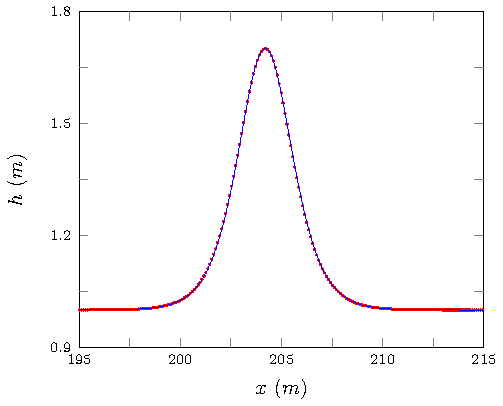
\includegraphics[width=\textwidth]{pics/results/soliton/ex/FDc.pdf}
\subcaption*{\hspace{10 mm}(a)}
\end{subfigure}
\begin{subfigure}{0.5\textwidth}
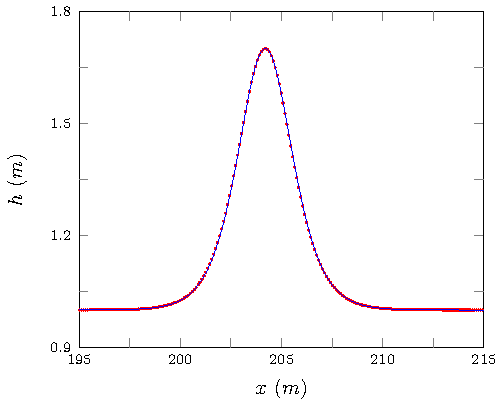
\includegraphics[width=\textwidth]{pics/results/soliton/ex/grim.pdf}
\subcaption*{\hspace{10 mm}(b)}
\end{subfigure}
\caption{Comparison between water profile of analytic solution ({\color{blue} \solidrule}) of the solitary wave problem \eqref{eq:sol} and numerical solution ({\color{red} $\bullet$}) with $\Delta x = 10/2^{12}m$ for $\mathcal{G}$ (a) and $\mathcal{E}$ (b) at $t=50s$.}
\label{fig:FDMsolexp}
\end{figure}
\begin{figure}
	\centering
	\begin{subfigure}{\textwidth}
		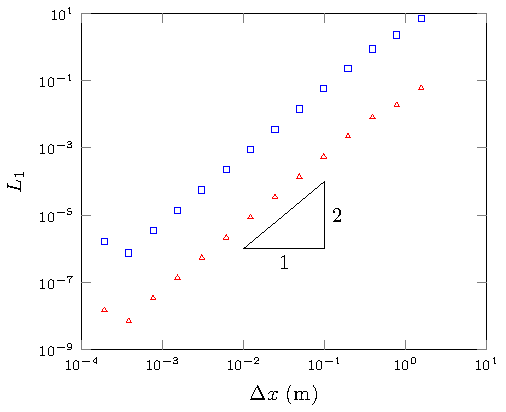
\includegraphics[width=0.5\textwidth]{pics/results/soliton/L1/FDc.pdf}
		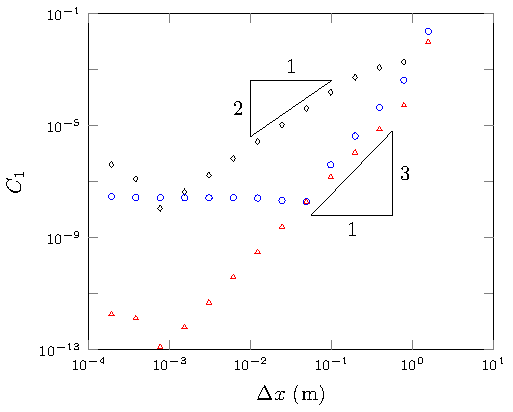
\includegraphics[width=0.5\textwidth]{pics/results/soliton/C1/FDc.pdf}
		\caption{}
	\end{subfigure}
	\begin{subfigure}{\textwidth}
		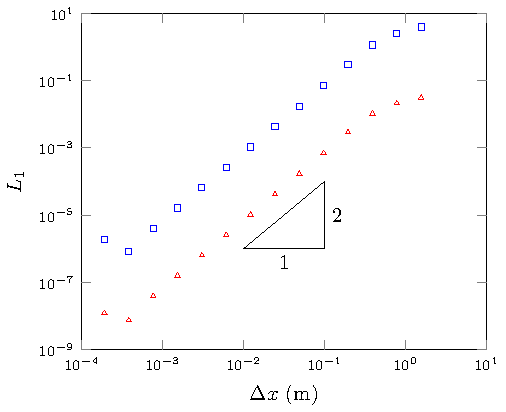
\includegraphics[width=0.5\textwidth]{pics/results/soliton/L1/grim.pdf}
		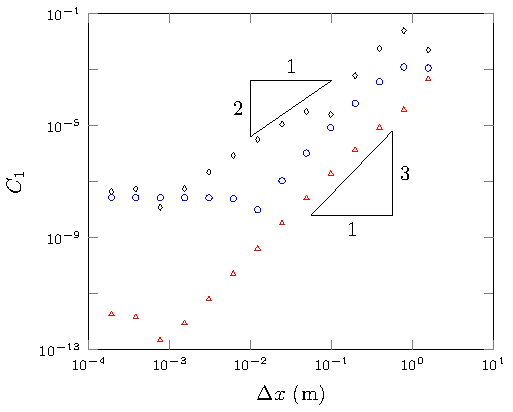
\includegraphics[width=0.5\textwidth]{pics/results/soliton/C1/grim.pdf}
		\caption{}
	\end{subfigure}
\caption{On the left $L_1$ for $h$ ({\color{red} $\triangle$}) and $u$ ({\color{blue} $\square$}) and on the right $C_1$ for $h$ ({\color{red} $\triangle$}), $uh$ ({\color{black} $\diamond$}) and $\mathcal{H}$ ({\color{blue} $\circ$}) for the numerical solution of the solitary wave problem by $\mathcal{G}$(a) and $\mathcal{E}$(b).}
\label{fig:FDMsolnorm}
\end{figure}
%

From Figure \ref{fig:FDMsolnorm} it can be seen that both finite difference methods are convergent under $L_1$ with second-order accuracy. There is however suboptimal rates of convergence for very small $\Delta x$ due to round off effects and suboptimal rates of convergence for large $\Delta x$ due to the initial conditions not being accurately represented on a coarse grid. Figure \ref{fig:FDMsolnorm} demonstrates conservation of mass, momentum and the Hamiltonian to at least second-order accuracy for both finite difference schemes. Both schemes conserve mass and momentum very well with round off error dominance occurring at the same place as for $L_1$. For $C_1$ of $\mathcal{H}$ the effects of round off errors occur earlier due to the greater number of calculations.

All of these measures demonstrate that $\mathcal{G}$ and $\mathcal{E}$ are appropriate to solve highly non-linear problems with smooth initial conditions for the Serre equations. 
%--------------------------------------------------------------------------------
\section{Smoothed Dam-Break}
\label{section:smootheddambreak}
%--------------------------------------------------------------------------------
The discontinuous dam-break problem can be approximated smoothly using the hyperbolic tangent function. Such an approximation will be called a smoothed dam-break problem and will be defined as such
\begin{linenomath*}
\begin{subequations}
\begin{gather}
h(x,0) = h_0 + \frac{h_1 - h_0}{2}\left(1 + \tanh\left(\frac{x_0 - x}{\alpha}\right)\right),
\end{gather}
\begin{gather}
u(x,0) = 0.0m/s.
\end{gather}
\label{eq:sdbi}
\end{subequations}
\end{linenomath*}
Where $\alpha$ measures the distance over which $46.117\%$ of the smooth transition between the two heights of $h_0$ and $h_1$ centered around $x_0$ occurs. Figure \ref{fig:dbsmoothinit} demonstrates the effect of varying $\alpha$ for the smoothed dam-break problem with $h_1 =1.8m$, $h_0 = 1m$ and $x_0 = 500m$. These are the same $h_0$ and $h_1$ values as those of the dam-breaks presented by \citeN{El-etal-2006} and \citeN{Hank-etal-2010-2034} and will be the values used throughout this paper.
\begin{figure}
\centering
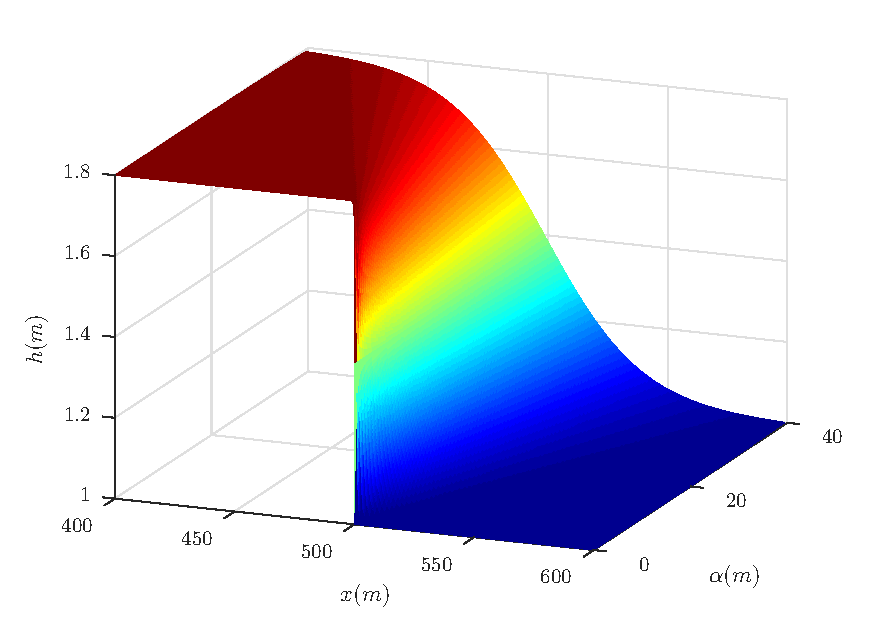
\includegraphics[width=0.6\textwidth]{pics/explainers/dbs.pdf}
\caption{Initial conditions for the smooth dam-break problem with $h_0 = 1m$, $h_1 = 1.8m$ and $x_0 =500m$ as $\alpha$ varies.}
\label{fig:dbsmoothinit}
\end{figure}
%

From \eqref{eq:sdbi} the following expressions for $C_{h}(0)$, $C_{uh}(0)$ and $C_{\mathcal{H}}(0)$ were derived provided $x_0$ is the midpoint of the spatial domain $\left[a,b \right]$ in which the smoothed dam-break occurs
\begin{linenomath*}
	\begin{subequations}
	\begin{gather*}
	\mathcal{C}_{h}(0) = \frac{h_1 + h_0}{2}\left(b- a\right),
	\label{eq:Chdef}
	\end{gather*}
	\begin{gather*}
	\mathcal{C}_{uh}(0) = 0
	\label{eq:Cuhdef}
	\end{gather*}
		and
	\begin{gather*}
	\mathcal{C}_{\mathcal{H}}(0) = \frac{g}{4} \left(h_0^2 - h_1^2 + \alpha\left(h_1 - h_0\right)^2\tanh\left(\frac{a - b}{2 \alpha}\right)\right).
	\label{eq:CHdef}
	\end{gather*}
		\label{eq:Canalyticvalues}	
	\end{subequations}
\end{linenomath*}
Note that due to a difference in heights at the two boundaries there is a flux of momentum into the system equal to $tg\left(h^2(b) - h^2(a)\right)$ and this must be accounted for in $C_1$ of $uh$.

The dam-break problem for the Serre equations results in the creation of an undular bore that is very similar to the analytic solution of the dam-break problem for the shallow water wave equations with oscillations \cite{Hank-etal-2010-2034,Dutykh-2014-315}. Because the analytic solution to the dam-break problem for the shallow water wave equations will be used as a reference in this paper we present it in Figure \ref{fig:SWWEanadiagram} for $h_0 = 1m$, $h_1 =1.8m$ and $x_0 = 500m$ at $t=30s$. The regions I through V in Figure \ref{fig:SWWEanadiagram} will be used to simplify our explanations later on for numerical solutions of the Serre equations. We also present equations for the quantities of interest in the analytic solution of the dam-break problem for the shallow water wave equations; the constant height ($h_2$) and velocity ($u_2$) in regions III and IV and the speed of the shock ($S_2$) which marks the boundary between regions IV and V.  From \citeN{Wu-etal-1999-1210} we have the following equations
\begin{linenomath*}
\begin{subequations}
\begin{gather}
h_2 = \frac{h_0}{2} \left[\sqrt{1 + 8 \left(\frac{2h_2}{h_2 - h_0}\frac{\sqrt{gh_1} - \sqrt{gh_2}}{\sqrt{gh_0}}\right)^2} - 1\right],
\end{gather}
	\begin{gather}
	u_2 = 2\left(\sqrt{gh_1} - \sqrt{gh_2}\right)
	\end{gather}
and
	\begin{gather}
	S_2 = \frac{h_2 u_2}{h_2 - h_0}.
	\end{gather}
\label{eq:WuSWWE}	
\end{subequations}
\end{linenomath*}
From these values we also define $x_{u_2}(t) = x_0 + u_2t$ and $x_{S_2}(t) = x_0 + S_2t$ to give the location of a fluid particle starting at $x_0$ travelling at speed $u_2$ and $S_2$ respectively at time $t$.

Undular bores for the one dimensional Serre equations were analysed by \citeN{El-etal-2006} and an expression for the amplitude ($A^+$) and speed ($S^+$) of the leading wave of a bore shown in Figure \ref{fig:Serreanadiagram} were given


\begin{linenomath*}
	\begin{subequations}
\begin{gather}
\frac{\Delta}{\left(A^+ + 1\right)^{1/4}} - \left(\frac{3}{4 -  \sqrt{A^+ + 1}}\right)^{21/10} \left(\frac{2}{1 + \sqrt{A^+ + 1}}\right)^{2/5} = 0
\label{eq:aplusdef}
\end{gather}
\begin{gather}
S^+ = \sqrt{g \left(A^+ + 1\right)}
\label{eq:splusdef}
\end{gather}
		\label{eq:ELWhitMod}	
	\end{subequations}
\end{linenomath*}
where $\Delta = h_b / h_0$, and $h_b$ is the amplitude of the bore. From this we define $x_{S^+}(t) = x_0 + S^+t$ which is the location of a fluid particle starting at $x_0$ and travelling at speed $S^+$ at time $t$.

\begin{figure}
\centering
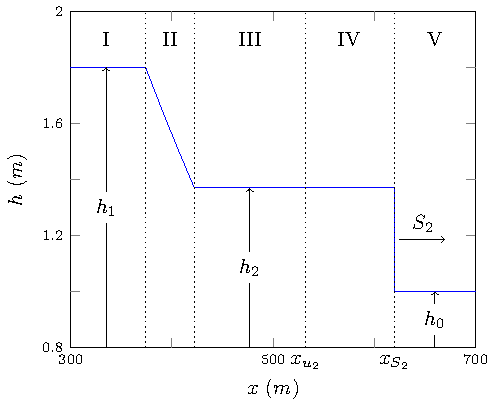
\includegraphics[width=0.5\textwidth]{pics/explainers/SWWEana.pdf}
\caption{Analytic solution at $t=30s$ of the shallow water wave equations for the dam-break problem with $h_0 = 1m$, $h_1=1.8m$ and $x_0=100m$.}
\label{fig:SWWEanadiagram}
\end{figure}

\begin{figure}
\centering
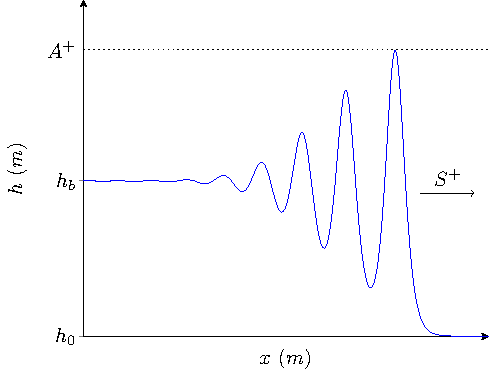
\includegraphics[width=0.5\textwidth]{pics/explainers/SERREex.pdf}
\caption{Demonstration of quantities obtained by Whitham modulation for undular bores of the Serre equations.}
\label{fig:Serreanadiagram}
\end{figure}
The simulations were run with various values of $\Delta x$ and $\alpha$. In regions III and IV there is a background flow and so $\mathcal{E}$ is unstable, to account for this the growth factor was suppressed by using a smaller time step than the CFL condition of $\Delta t = 0.01 \Delta x$. $\mathcal{V}_2$ requires an input parameter to its slope limiter and this was chosen to be $\theta = 1.2$ \cite{Zoppou-etal-2017}. 
%[cite ASCE?] [] 
The first set of scenarios presented were run until $t=30s$ on the interval $x\in[0m,1000m]$.

Applying \eqref{eq:WuSWWE} to our dam-break problem results in $h_2 = 1.36898m$ , $u_2 = 1.074975$ $m/s$ and $S_2 = 3.98835$ $m/s$ which can be seen in Figure \ref{fig:SWWEanadiagram}. For \eqref{eq:ELWhitMod} as in \citeN{El-etal-2006} the height of the bore is given as
\begin{gather*}
\label{eqn:hrdef}
h_b = \frac{\left(\sqrt{\frac{h_1}{h_0}} + 1\right)^2}{4}.
\end{gather*} 
Thus $h_b = 1.37082$ $m$, $\Delta = 1.37082$,  $A^+ = 1.73998$ $m$ and $S^+ = 4.13148$ $m/s$.
Note that due to the different natures of bores for the Serre and shallow water wave equations $S^+ \neq S_2$.

%%%
%% DOWN HERE 
%%	
%%

%--------------------------------------------------------------------------------
\subsection{Results}
%--------------------------------------------------------------------------------

%Intro
We begin this study by looking into the effect of the initial steepness of the smoothed dam-break problem for different $\alpha$ values by observing what happens as $\Delta x \rightarrow 0$ and our numerical solution better approximates the true solution of the Serre equations. To have the smallest error we use the highest order well validated model $\mathcal{V}_3$ in the following investigation. From these results we then investigate numerical results for long time scales, how the shallow water wave equations analytic solution and El's Whitham modulation values compare to our results and then finally present some other findings about the behaviour of our numerical solutions.

\subsubsection{Effect of $\alpha$}
Because the smoothing process is a non-physical numerical tool we first study its effect by decreasing $\alpha$ and thus better approximating the dam-break. To do this we fix an $\alpha$ and then investigate the numerical solutions as $\Delta x \rightarrow 0$ and our well validated numerical method better approximates the true solution of the Serre equations. 

The first observation is that there are four types of behaviour as $\Delta x \rightarrow 0$ depending on the $\alpha$ and the numerical method. The four behaviours are identified by the nature of the solutions around $x_{u_2}$ when $\Delta x$ is small and they correspond to different results presented in the literature. For brevity the only given examples of these behaviours will be the solutions of $\mathcal{V}_3$ although they all also occurred for the $\mathcal{E}$, $\mathcal{G}$ and $\mathcal{V}_2$ simulations using the same $\alpha$ and $\Delta x = 10/2^{10}m$.

The first behaviour which will be referred to as the non-oscillatory behaviour has such smooth initial conditions that no oscillations were introduced by $t= 30s$ for the numerical simulations, although given sufficient time the front steepens and an undular bore will develop. This behaviour is not present in the literature as no authors chose large enough $\alpha$ values. An example of this behaviour can be seen in Figure \ref{fig:o3a1dxlimflatexp} for $\alpha = 40m$. Because this is a very smooth problem we observe that all numerical results are visually identical for all $\Delta x < 10 / 2^4m$. We observed this behaviour for $\mathcal{V}_1$'s simulations as well. We note that $\mathcal{V}_3$'s numerical solution has $h(x_{u_2}) > h_2$ and because no undulations are present \citeN{El-etal-2006} results are not applicable to these solutions.   

Convergence is also present in Figure \ref{fig:o3a1dxlimmeasure} with both the $L_1$ and $C_1$ measures. Here $L_1$ has been modified to use the numerical solution when $\Delta x = 10 / 2^{10}m$ as an approximation to the analytic solution because none are currently known for the Serre equations. For $L_1$ and $C_1$ of $\mathcal{H}$ the order of accuracy is the theoretical one. Since $L_1$ compares only numerical results, round-off errors result in error stagnation rather than increase as in Figure \ref{fig:FDMsolnorm}. $C_1$ for $h$ demonstates that the finite volume method does indeed conserve mass independent of $\Delta x$ with round-off errors dominant for all tested $\Delta x$. $C_1$ of $uh$ has been omitted because there is a small but noticable flux of momentum at the boundaries due to the large $\alpha$, which dominates the errors and cannot be accounted for. The presented measures suggest that this family of solutions is an accurate representation of the behaviour of the Serre equations when $\alpha$ is sufficiently large and in particular $\alpha = 40m$. 


\begin{figure}
\centering
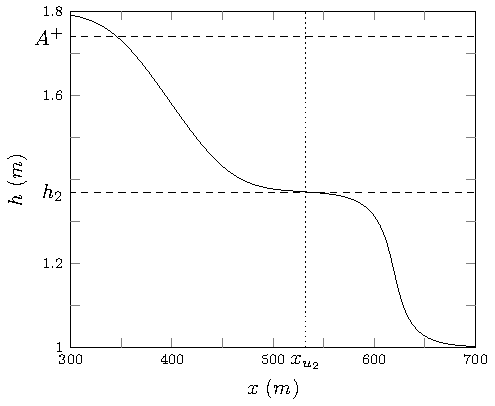
\includegraphics[width=0.7\textwidth]{pics/results/SDB/numsols/alpha0.025/1-figure0.pdf}
\caption{Numerical results of $\mathcal{V}_3$  at $t= 30s$ for the smooth dam-break problem with $\alpha = 40m$ for $\Delta x = 10/2^{4}m$ ({\color{black} \solidrule}).}
\label{fig:o3a1dxlimflatexp}
\end{figure}
%
\begin{figure}
\centering
\begin{subfigure}{\textwidth}
	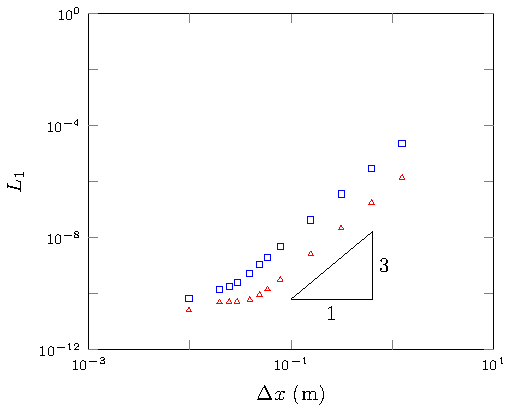
\includegraphics[width=0.5\textwidth]{pics/results/SDB/Lcon/alpha0.025/1.pdf}
	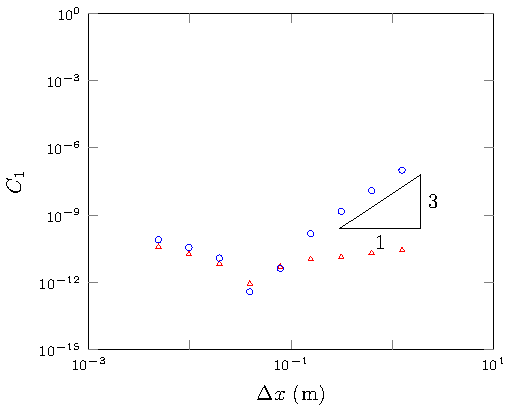
\includegraphics[width=0.5\textwidth]{pics/results/SDB/Con/1.pdf}
\end{subfigure}
\caption{On the left is $L_1$ for $h$ ({\color{red} $\triangle$}) and $u$ ({\color{blue} $\square$}) and on the right is $C_1$ for $h$ ({\color{red} $\triangle$}) and $\mathcal{H}$ ({\color{blue} $\circ$}) for $\mathcal{V}_3$'s solution for the smooth dam-break problem with $\alpha = 40m$.}
\label{fig:o3a1dxlimmeasure}
\end{figure}

The second behaviour will be referred to as the flat behaviour due to the presence of a constant height around $x_{u_2}$, this is the most common behaviour observed in the literature \cite{Hank-etal-2010-2034,Dutykh-2014-315,Mitsotakis-etal-2014}. This behaviour has oscillations in regions III and IV which are seperated by a constant height state around $x_{u_2}$. An example of the numerical results for this behaviour can be seen in Figure \ref{fig:o3a6dxlimflatexp} when $\alpha = 2m$.

As $\Delta x$ decreases the solutions converge so that by $\Delta x = 10 / 2^8m$ the solutions for higher $\Delta x$ are visually identical. There is also good agreement between the peak amplitude in region IV ($A$) and $A^+$ as well as $h(x_{u_2})$ and $h_2$. Although as $\Delta x$ is decreased in the simulations we observe $h(x_{u_2}) > h_2$. Since this method is well validated for smooth problems and a small $\Delta x$ has been chosen this suggests that the mean bore heights in regions III and IV from a dam-break may differ slightly between the shallow water wave equations and the Serre equations. These results also compare well to the results in \citeN{Mitsotakis-etal-2014} who use the same $\alpha$ but different $h_0$ and $h_1$. We observed this behaviour for $\mathcal{V}_1$'s simulations.

The measures $L_1$ and $C_1$ demonstrate good convergence with the expected order of accuracy. For $\mathcal{V}_3$ we observe that $C_1$ of $uh$ has a larger error but a higher order of accuracy than $C_1$ of $\mathcal{H}$. The higher order of accuracy makes sense as the conversion between the conserved quantity $G$ and $u$ is fourth order. The smaller $C_1$ error of $\mathcal{H}$ can be explained by noting that although $uh$ is a component of $\mathcal{H}$, $gh^2$ makes up a far larger portion of $\mathcal{H}$ see Figure \ref{fig:PHTa12all}, diminishing the relative size of the $uh$ errors in $\mathcal{H}$.
%C_1  of G is C_1 of uh is u(a) = u(b) = 0

These results demonstrate that this behaviour is an accurate representation of the nature of the Serre equations provided $\alpha$ is large enough supporting the findings of \citeN{Mitsotakis-etal-2014}.

\begin{figure}
\centering
\begin{subfigure}{\textwidth}
	\centering
	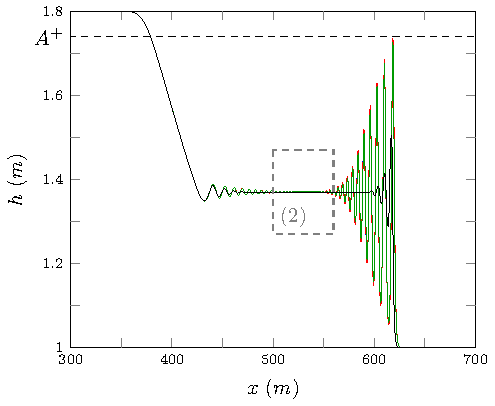
\includegraphics[width=0.7\textwidth]{pics/results/SDB/numsols/alpha0.5/1-figure0.pdf}
\end{subfigure}
\begin{subfigure}{\textwidth}
	\centering
	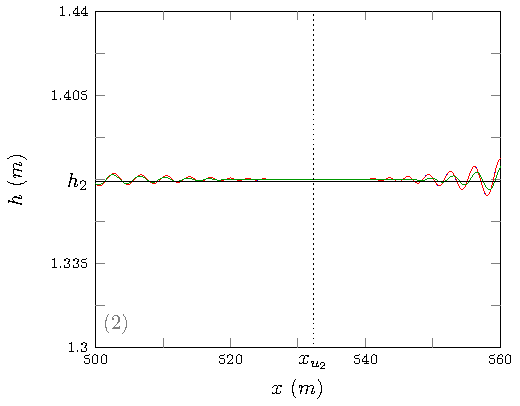
\includegraphics[width=0.5\textwidth]{pics/results/SDB/numsols/alpha0.5/2-figure0.pdf}
\end{subfigure}
\caption{Numerical results of $\mathcal{V}_3$  at $t= 30s$ for the smooth dam-break problem with $\alpha = 2m$ for $\Delta x = 10/2^{10}m$ ({\color{blue} \solidrule}), $10/2^8m$ ({\color{red} \solidrule}), $10/2^6m$ ({\color{green!60!black} \solidrule}) and $10/2^{4}m$ ({\color{black} \solidrule}).}
\label{fig:o3a6dxlimflatexp}
\end{figure}

\begin{figure}
	\centering
\begin{subfigure}{\textwidth}
	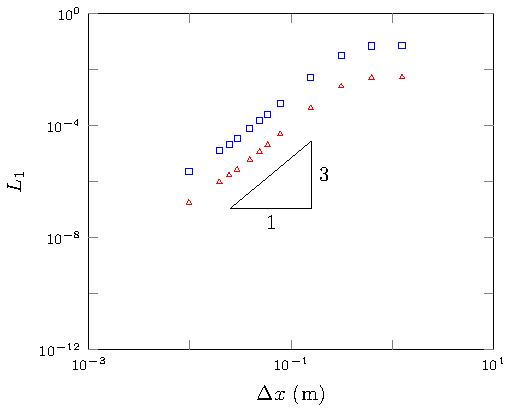
\includegraphics[width=0.5\textwidth]{pics/results/SDB/Lcon/alpha0.5/1.pdf}
	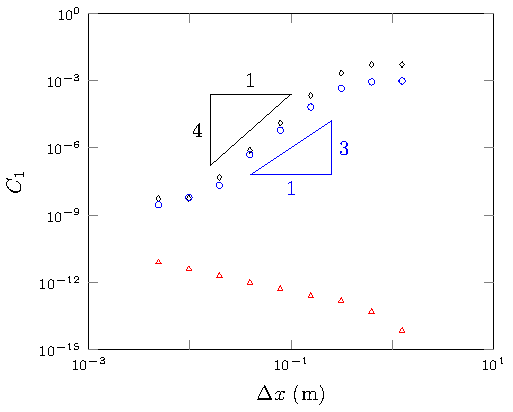
\includegraphics[width=0.5\textwidth]{pics/results/SDB/Con/6.pdf}
\end{subfigure}
	\caption{On the left is $L_1$ for $h$ ({\color{red} $\triangle$}) and $u$ ({\color{blue} $\square$}) and on the right is $C_1$ for $h$ ({\color{red} $\triangle$}), $uh$ ({\color{black} $\diamond$}) and $\mathcal{H}$ ({\color{blue} $\circ$}) for $\mathcal{V}_3$'s solution for the smooth dam-break problem with $\alpha = 2m$.}
	\label{fig:o3a2dxlimmeasure}
\end{figure}

The third behaviour will be referred to as the node behaviour and it is was observed by \citeN{El-etal-2006}. The node behaviour's main feature is that the oscillations in region III and IV decay and appear to meet at $x_{u_2}$ as can be seen in Figure \ref{fig:o3a9dxlimcdexp} when $\alpha = 0.4m$. All the methods have not converged to a solution as $\Delta x$ decreases. However, it does appear that convergence is likely with the solutions getting closer together. This is expected for the smaller $\Delta x$ because the problem is still smooth. In these results $A^+$ is a good estimator for $A$ and the oscillations in regions III and IV appear to be around $h_2$. This behaviour was observed by \citeN{El-etal-2006} for $\mathcal{E}$ and indeed we have replicated it for all the high order methods. It was not observed in $\mathcal{V}_1$'s solutions up to $\Delta x=10/2^{10}m$ with $\alpha=0.001m$ as $\mathcal{V}_1$ introduces diffusive errors that severly dampen the oscillations. This explains why \citeN{Hank-etal-2010-2034} using $\mathcal{V}_1$ could not replicate the results of \citeN{El-etal-2006}. It was found that an $\alpha$ of at least $0.4m$ is required to recover the node behaviour this explains why \citeN{Mitsotakis-etal-2014} and \citeN{Dutykh-2014-315} using $\alpha$'s of $2m$ and $1m$ respectively could not replicate the results of \citeN{El-etal-2006}. 

The assertion that these results are close to converging to a solution is supported by Figure \ref{fig:o3a3dxlimmeasure} with appropriate orders of accuracy for $L^*_1$ and $C_1$. Figure \ref{fig:o3a9dxlimcdexp} demonstrates that the final solutions have not yet converged, thus we modify $L_1$ to omit $[520m,540m]$ and call this modified measure $L^*_1$. $L^*_1$ demonstrates that even though the section around $x_{u_2}$ has not been fully resolved we do see that there is convergence at the appropriate order away from $x_{u_2}$. This suggests that the effect of better resolving the oscillations will only be felt locally. $C_1$ demonstrates the appropriate order of accuracy in conserving momentum and the Hamiltonian suggesting that we are indeed approaching a reasonable solution to this problem as $\Delta x$ is decreased. 

These results demonstrate that although we have not yet fully converged this behaviour is close to reasonable solutions of the Serre equations given the appropriate $\alpha$ value supporting the findings of \citeN{El-etal-2006}.
\begin{figure}
\centering
\begin{subfigure}{\textwidth}
	\centering
	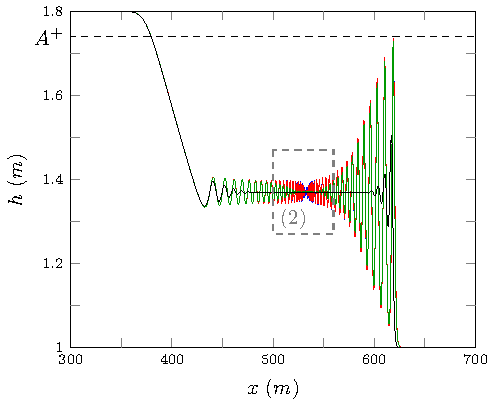
\includegraphics[width=0.7\textwidth]{pics/results/SDB/numsols/alpha2.5/1-figure0.pdf}
\end{subfigure}
\begin{subfigure}{\textwidth}
	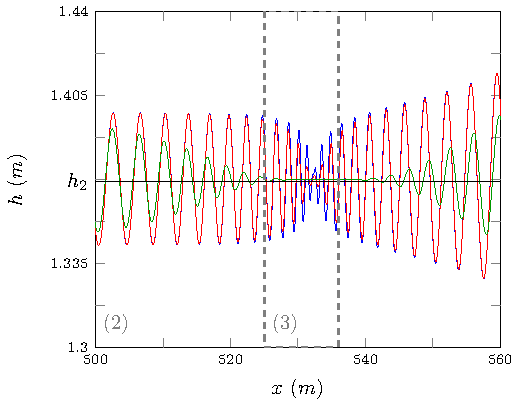
\includegraphics[width=0.5\textwidth]{pics/results/SDB/numsols/alpha2.5/2-figure0.pdf}
	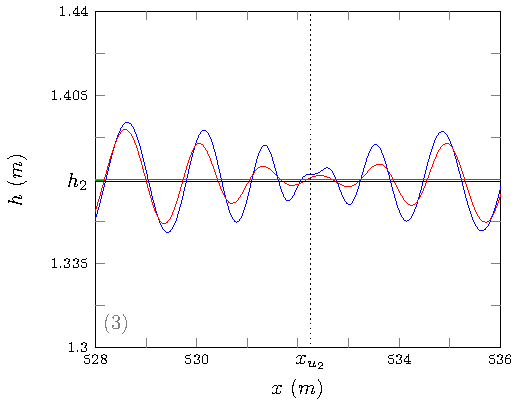
\includegraphics[width=0.5\textwidth]{pics/results/SDB/numsols/alpha2.5/3-figure0.pdf}
\end{subfigure}
\caption{Numerical results of $\mathcal{V}_3$  at $t= 30s$ for the smooth dam-break problem with $\alpha = 0.4m$ for $\Delta x = 10/2^{10}m$ ({\color{blue} \solidrule}), $10/2^8m$ ({\color{red} \solidrule}), $10/2^6m$ ({\color{green!60!black} \solidrule}) and $10/2^{4}m$ ({\color{black} \solidrule}).}
\label{fig:o3a9dxlimcdexp}
\end{figure}


\begin{figure}
	\centering
	\begin{subfigure}{\textwidth}
		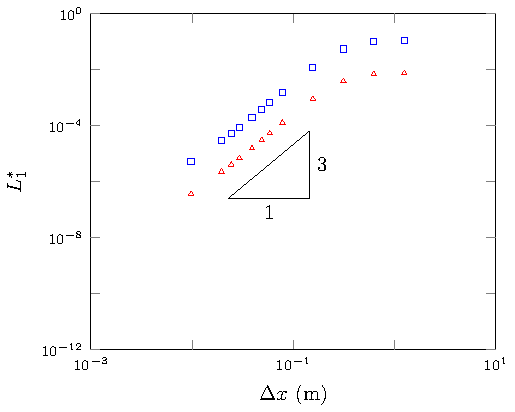
\includegraphics[width=0.5\textwidth]{pics/results/SDB/Lcon/alpha2.5/1.pdf}
		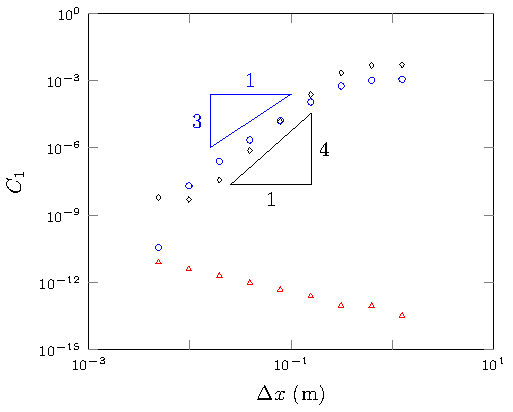
\includegraphics[width=0.5\textwidth]{pics/results/SDB/Con/9.pdf}
	\end{subfigure}
	\caption{On the left is $L^*_1$ for $h$ ({\color{red} $\triangle$}) and $u$ ({\color{blue} $\square$}) and on the right is $C_1$ for $h$ ({\color{red} $\triangle$}), $uh$ ({\color{black} $\diamond$}) and $\mathcal{H}$ ({\color{blue} $\circ$}) for $\mathcal{V}_3$'s solution for the smooth dam-break problem with $\alpha = 0.4m$.}
	\label{fig:o3a3dxlimmeasure}
\end{figure}


The fourth behaviour will be referred to as the bump behaviour due to the oscillations no longer decaying down towards a point but rather growing around $x_{u_2}$ forming a bump as can be seen in Figure \ref{fig:o3a20dxlimcdexp} for $\alpha = 0.1m$. This behaviour has hitherto not been published and is certainly not an expected result. 

This behaviour is even further from converging with decreasing $\Delta x$ around $x_{u_2}$ than the node behaviour as can be seen in Figure \ref{fig:o3a20dxlimcdexp}. $L^*_1$ demonstrates good convergence outside this middle region as can be seen in Figure \ref{fig:o3a4dxlimmeasure} so that resolving the region around $x_{u_2}$ is the main difficulty for our numerical methods. $C_1$ of $uh$ and $\mathcal{H}$ also converges but compared to the other behaviours we have lost an order of accuracy in these measures. This suggests that we are not using the appropriate $\Delta x$ and thus smaller grids are required to attain the appropriate order of convergence for $\mathcal{V}_3$. Because, convergence is not assured by these numerical results there is the possibility that the wave amplitudes around the $x_{u_2}$ could grow rapidly. This however has not been observed, with numerical results where $\alpha = 0.001m$ and $\Delta x = 10.0/ 2^{10}m$ at which point the initial conditions are basically a discontinuous dam-break showing an increase but not a large growth in the amplitude of the bump for $\mathcal{V}_3$.

\begin{figure}
\centering
\begin{subfigure}{\textwidth}
	\centering
	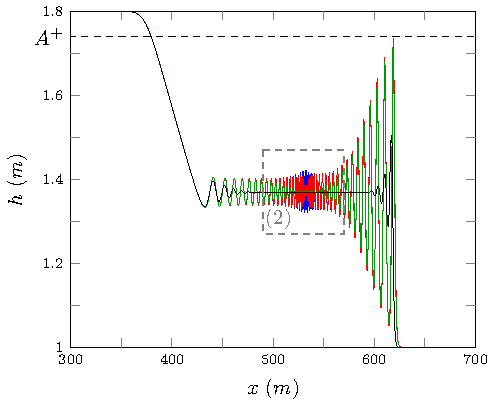
\includegraphics[width=0.7\textwidth]{pics/results/SDB/numsols/alpha10/1-figure0.pdf}
\end{subfigure}
\begin{subfigure}{\textwidth}
	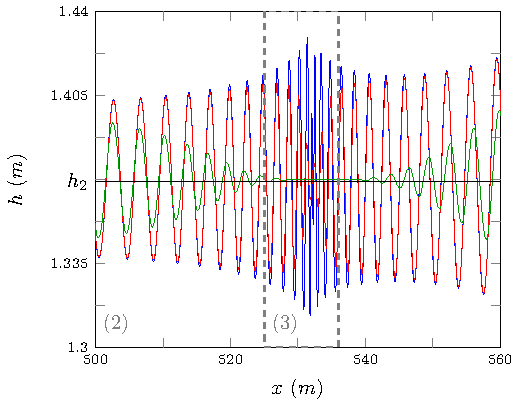
\includegraphics[width=0.5\textwidth]{pics/results/SDB/numsols/alpha10/2-figure0.pdf}
	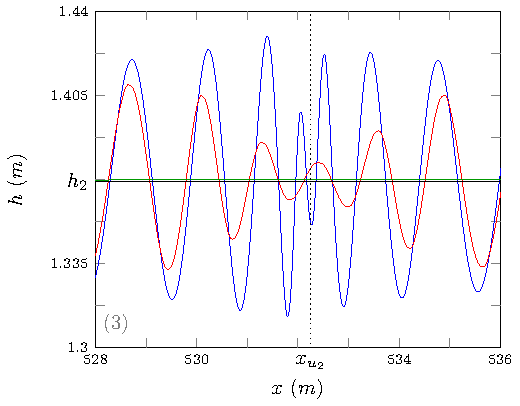
\includegraphics[width=0.5\textwidth]{pics/results/SDB/numsols/alpha10/3-figure0.pdf}
\end{subfigure}
\caption{Numerical results of $\mathcal{V}_3$  at $t= 30s$ for the smooth dam-break problem with $\alpha = 0.1m$ for $\Delta x = 10/2^{10}m$ ({\color{blue} \solidrule}), $10/2^8m$ ({\color{red} \solidrule}), $10/2^6m$ ({\color{green!60!black} \solidrule}) and $10/2^{4}m$ ({\color{black} \solidrule}).}
\label{fig:o3a20dxlimcdexp}
\end{figure}

\begin{figure}
	\centering
	\begin{subfigure}{\textwidth}
		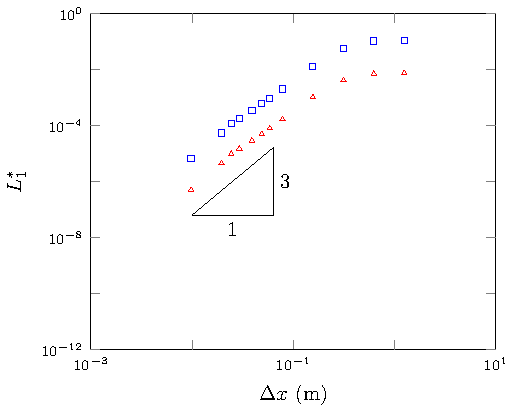
\includegraphics[width=0.5\textwidth]{pics/results/SDB/Lcon/alpha10/1.pdf}
		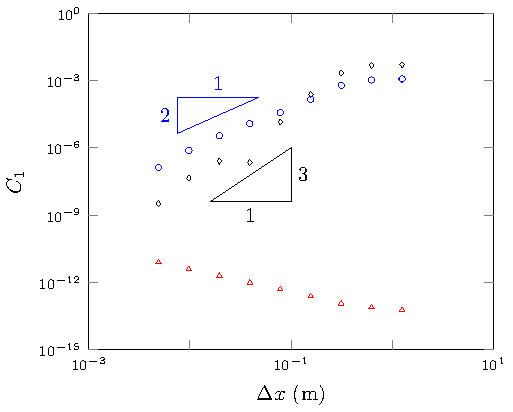
\includegraphics[width=0.5\textwidth]{pics/results/SDB/Con/12.pdf}
	\end{subfigure}
	\caption{On the left is $L^*_1$ for $h$ ({\color{red} $\triangle$}) and $u$ ({\color{blue} $\square$}) and on the right is $C_1$ for $h$ ({\color{red} $\triangle$}), $uh$ ({\color{black} $\diamond$}) and $\mathcal{H}$ ({\color{blue} $\circ$}) for $\mathcal{V}_3$'s solution for the smooth dam-break problem with $\alpha = 0.1m$.}
	\label{fig:o3a4dxlimmeasure}
\end{figure}


% % % % % % % % % % % % % % % % % % % % MOST WORK DOWN HERE!!!! % % % % % % % % % % % % % % % % % % % % % %
% % % % % % % % % % % % % % % % % % % % % %% % % % % % % % % % % % % % % % % % % % % %% % % % % % % % % % %
% % % % % % % % % % % % % % % % % % % % % %% % % % % % % % % % % % % % % % % % % % % %% % % % % % % % % % %
% % % % % % % % % % % % % % % % % % % % % %% % % % % % % % % % % % % % % % % % % % % %% % % % % % % % % % %
% % % % % % % % % % % % % % % % % % % % % %% % % % % % % % % % % % % % % % % % % % % %% % % % % % % % % % %
% % % % % % % % % % % % % % % % % % % % % %% % % % % % % % % % % % % % % % % % % % % %% % % % % % % % % % %

%smoothing for El as well
%add S_2

Since this result is unexpected and not as supported as the node behaviour in the literature \cite{El-etal-2006}. The first check should be different numerical methods such as $\mathcal{G}$ and $\mathcal{E}$ to test if some numerical effect from the reformulation of the Serre equations or the elliptic solver are the cause. For comparison $\mathcal{G}$, $\mathcal{E}$, $\mathcal{V}_1$ and $\mathcal{V}_3$ are applied to the same initial conditions with the same grid resolutions as above and the results were plotted in Figure \ref{fig:MODlim}. $\mathcal{V}_2$ has been omitted from this figure for clarity because its solution is very close to $\mathcal{V}_3$ as noted by \citeN{Zoppou-etal-2017}. The first observation is that $\mathcal{V}_1$ has not recovered this behaviour. This is because $\mathcal{V}_1$ is very diffusive \cite{Zoppou-etal-2017}, dampening these oscillations. To resolve such behaviour for $\mathcal{V}_1$ would require very small $\Delta x$ and as such this has not been observed in the simulations. Secondly, all high-order methods recover this bump behaviour and disagree only in the region around $x_{u_2}$. The main difference in the oscillations is their phase and amplitude with the dispersive finite difference methods resulting in larger waves than the diffusive finite difference-volume hybrid methods. We also observe oscillations in $\mathcal{E}$ that are not replicated by the other methods close to $x_{u_2}$, this is caused by the instability of $\mathcal{E}$ with its effects being more obvious here due to the high frequency of these waves which correspond to larger growth factors. 

Since $\mathcal{V}_3$ is diffusive as can be seen in Figure \ref{fig:o3a20dxlimcdexp} and $\mathcal{G}$ is dispersive the true analytic solution should exist between $\mathcal{V}_3$ and $\mathcal{G}$, which is a bounded bump around $x_{u_2}$. $\mathcal{G}$ well approximates the Serre equations, although $\mathcal{V}_2$ and $\mathcal{V}_3$ are still preferred by the authors due to their robustness and superior conservation of quantities. 

\begin{figure}
\centering
\begin{subfigure}{\textwidth}
	\centering
	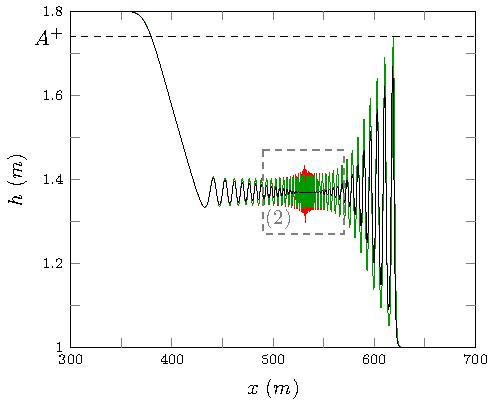
\includegraphics[width=0.7\textwidth]{pics/results/SDB/numsols/modelcomppalpha10dx10/1-figure0.pdf}
\end{subfigure}
\begin{subfigure}{\textwidth}
	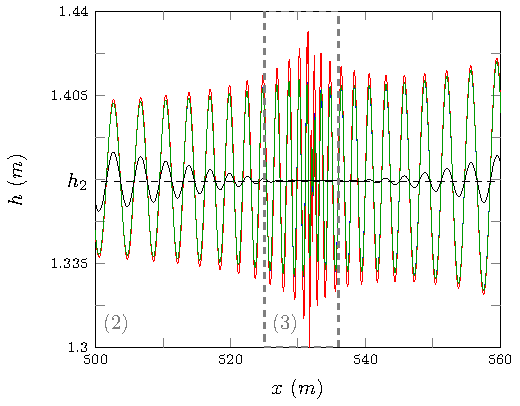
\includegraphics[width=0.5\textwidth]{pics/results/SDB/numsols/modelcomppalpha10dx10/2-figure0.pdf}
	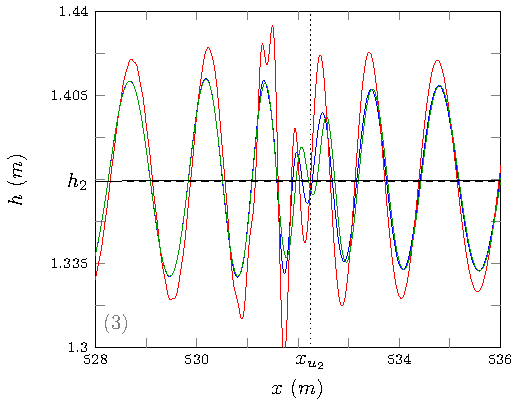
\includegraphics[width=0.5\textwidth]{pics/results/SDB/numsols/modelcomppalpha10dx10/4-figure0.pdf}
\end{subfigure}
\caption{Numerical results for the smooth dam-break problem with $\alpha = 0.1m$ and $\Delta x = 10/2^{10}m$
for $\mathcal{G}$ ({\color{blue} \solidrule}), $\mathcal{E}$ ({\color{red} \solidrule}), $\mathcal{V}_3$ ({\color{green!60!black} \solidrule}) and $\mathcal{V}_1$ ({\color{black} \solidrule}).}
\label{fig:MODlim}
\end{figure}

%\begin{figure}
%\centering
%\begin{subfigure}{\textwidth}
%	\centering
%	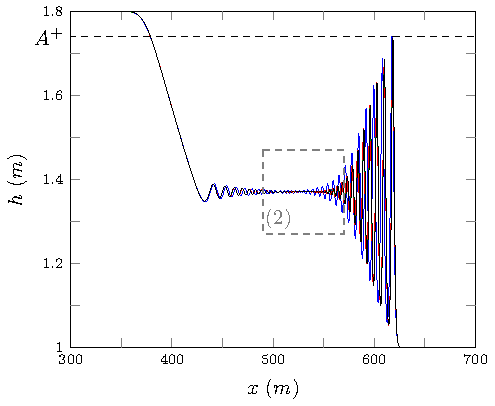
\includegraphics[width=0.7\textwidth]{pics/results/SDB/numsols/FDcalpha0.5/1-figure0.pdf}
%\end{subfigure}
%\begin{subfigure}{\textwidth}
%	\centering
%	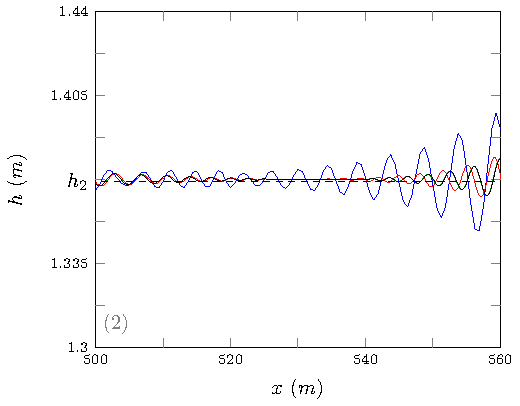
\includegraphics[width=0.5\textwidth]{pics/results/SDB/numsols/FDcalpha0.5/2-figure0.pdf}
%\end{subfigure}
%\caption{Numerical results of $\mathcal{G}$  at $t= 30s$ for the smooth dam-break problem with $\alpha = 2m$ for $\Delta x = 10/2^{4}m$ ({\color{blue} \solidrule}), $10/2^6m$ ({\color{red} \solidrule}), $10/2^8m$ ({\color{green!60!black} \solidrule}) and $10/2^{10}m$ ({\color{black} \solidrule}).}
%\label{fig:FDa6lim}
%\end{figure}

There is still the possibility that these solutions are caused by some numerical phenomena, more research into this topic should be undertaken. However, the agreement of all the discussed methods of sufficiently high order indicates that these results are representative of actual solutions of the smoothed dam-break problem with low $\alpha$ for the Serre equations. Lastly the bump behaviour was observed using $\mathcal{E}$ with a similar order of magnitude for $\Delta x$ and $\Delta t$ as \citeN{El-etal-2006}. The absence of a bump behaviour in their findings is caused by the smoothing of the initial conditions which is absent from the paper but was confirmed later by \citeN{El-Hoefer-2016-11}.

This concludes the explanation of how our results fit in with the current literature and the following section of this paper will be concerned with some further numerical investigation into these results. 


%--------------------------------------------------------------------------------
\subsubsection{Long time}\label{subsubsec:LT}
%--------------------------------------------------------------------------------
The first test of these results will be of its evolution through time, thus an experiment was run with the same parameters on a larger domain with $x \in [-900m, 1800m]$ for $t \in [0,300s]$. The results of $\mathcal{V}_3$ with $\alpha = 0.1m$ and $\Delta x = 10/2^{9}m$ and $10/2^{8}m$  at $t = 300s$ are presented in Figure \ref{fig:FVcomplonga20}. For this problem these parameters result in the bump behaviour as can be seen in Figure \ref{fig:o3a20dxlimcdexp}, however after sufficient time we can see that this bump behaviour has decayed back into a flat behaviour although there are still small oscillations present in the middle region. 

We also observe that $A^+$ has not been perfectly replicated with the numerical solution having larger peak amplitudes in region IV than $A^+$. Consequently we can see that while $x_{S^+}$ is a better approximation than $x_{S_2}$ to the position of the bore it is still an underestimate. Thus our bores will arrive a little earlier than predicted by $S^+$ and much earlier than predicted by $S_2$. We also note that as above the bore heights for the Serre and shallow water wave equations appear to be slightly different.

To track the decaying of the oscillations for $\mathcal{V}_3$'s solution around $x_{u_2}$ a snapshot of the area around $x_{u_2}$ has been plotted for different times in Figure \ref{fig:FVlongcemt500}. It can be seen that at $t =30s$ the solution exhibits the bump behaviour but as time progresses the region around $x_{u_2}$ has decayed into the node behaviour by $t=100s$ and then into the flat behaviour observed at $t=200s$ and $t=300s$. This could be a property of the solution of the Serre equations after sufficient time or due to the accumulation of diffusive errors of the numerical method with Figure \ref{fig:FVcomplonga20} demonstrating that over this time span we are not close to convergence of the numerical results. We note that \citeN{El-etal-2006} had very similar results in this longer time scale although their paper uses the normalised Serre equations so that in effect $g=1m/s^2$ and an unknown smoothing of the initial conditions which make comparisons of the solutions at similar times difficult.   

%coarsefinecomparison
\begin{figure}
	\centering
	\begin{subfigure}{\textwidth}
		\centering
		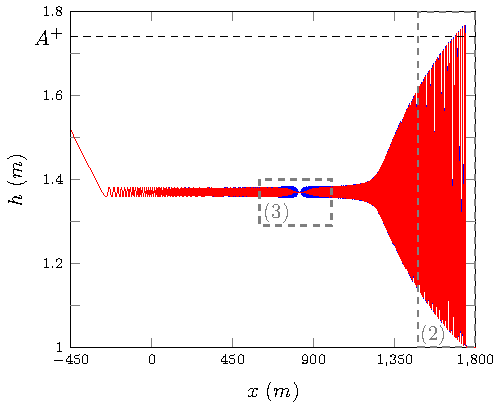
\includegraphics[width=0.7\textwidth]{pics/results/SDB/numsols/300s/CF0t300s.pdf}
	\end{subfigure}
	\begin{subfigure}{\textwidth}
		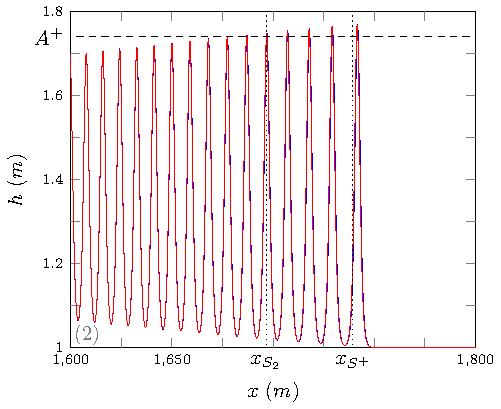
\includegraphics[width=0.5\textwidth]{pics/results/SDB/numsols/300s/CF1t300s.pdf}
		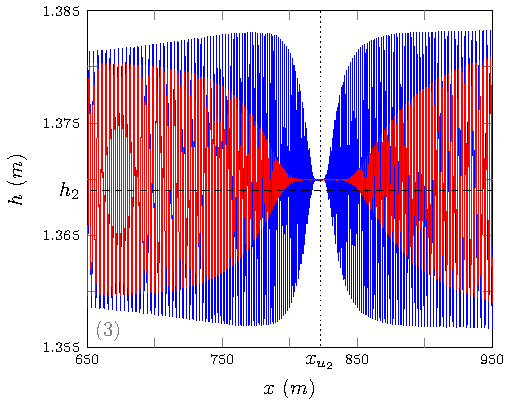
\includegraphics[width=0.5\textwidth]{pics/results/SDB/numsols/300s/CF2t300s.pdf}
	\end{subfigure}
	\caption{Numerical solution of smooth dam-break problem at $t=300s$ by $\mathcal{V}_3$ with $\alpha = 0.1m$ for $\Delta x = 10/2^{9}m$ ({\color{blue} \solidrule}) and $10/2^{8}m$ ({\color{red} \solidrule}).}
	\label{fig:FVcomplonga20}
\end{figure}

\begin{figure}
\centering
\begin{subfigure}{0.5\textwidth}
	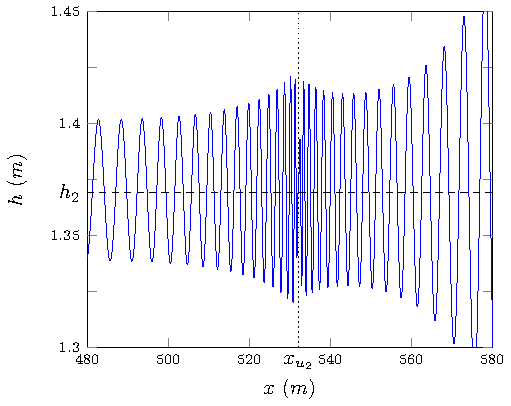
\includegraphics[width=\textwidth]{pics/results/SDB/numsols/300s/evolve30s.pdf}
	\subcaption*{\hspace{10 mm}$t=30s$}
\end{subfigure}%
\begin{subfigure}{0.5\textwidth}
	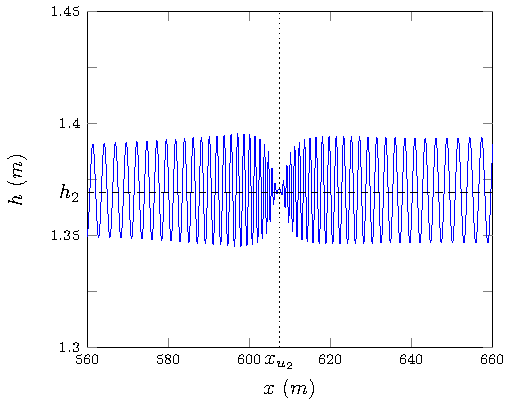
\includegraphics[width=\textwidth]{pics/results/SDB/numsols/300s/evolve100s.pdf}
	\subcaption*{\hspace{10 mm} $t=100s$}
\end{subfigure}
\begin{subfigure}{0.5\textwidth}
	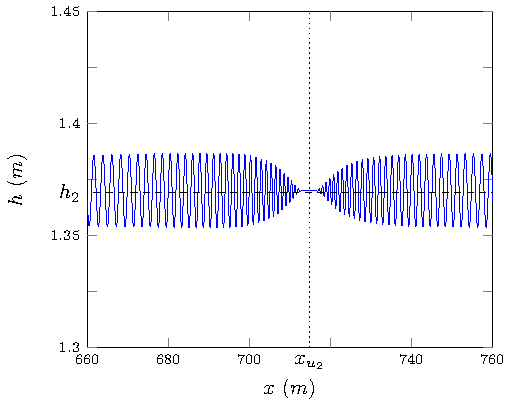
\includegraphics[width=\textwidth]{pics/results/SDB/numsols/300s/evolve200s.pdf}
	\subcaption*{\hspace{10 mm}$t=200s$}
\end{subfigure}%
\begin{subfigure}{0.5\textwidth}
	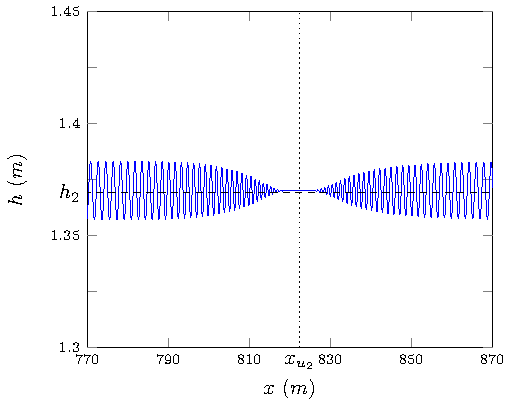
\includegraphics[width=\textwidth]{pics/results/SDB/numsols/300s/evolve300s.pdf}
	\subcaption*{\hspace{10 mm}$t=300s$}
\end{subfigure}

\caption{Numerical solution of the smooth dam-break problem by $\mathcal{V}_3$ with $\alpha = 0.1m$ and $\Delta x = 10/2^{9}m$ at various times.}
\label{fig:FVlongcemt500}
\end{figure}


\subsubsection{Shallow water wave equation comparison}
Since the shallow water wave equations have been used as a guide for the mean behaviour of the solution of the Serre equations in the literature \cite{Hank-etal-2010-2034,Mitsotakis-etal-2014} we would like to investigate how useful they are. 
%uh comparison
We first plot $h - h_2$ and $u - u_2$ for the smoothed dam-break problem with $\alpha = 0.1m$ and $\Delta x = {10}/{2^9}m$ in Figure \ref{fig:UHSWWcomp30sall} for $t= 30s$ and Figure \ref{fig:UHSWWcomp300sall} for $t= 300s$. From this we can see that over short time spans both $h_2$ and $u_2$ are good approximations to the mean behaviour of the fluid with both plots oscillating around $0$. However after sufficient time we see that the mean velocity and height of the fluid have diverged slightly from the shallow water wave equation values $h_2$ and $u_2$. With $h_2$ being an underestimate and $u_2$ being an overestimate. From Figure \ref{fig:FVcomplonga20} it can also be seen that $S_2$ underestimates the speed of the bore front.

\begin{figure}
	\centering
	\begin{subfigure}{\textwidth}
		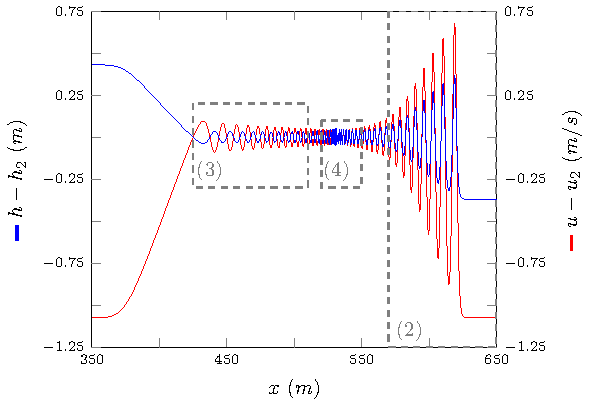
\includegraphics[width=0.5\textwidth]{pics/results/SDB/numsols/SWWCOMP/30s/0.pdf}
		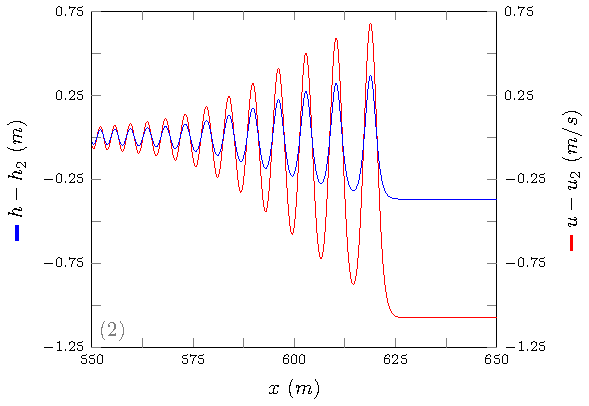
\includegraphics[width=0.5\textwidth]{pics/results/SDB/numsols/SWWCOMP/30s/2.pdf}
	\end{subfigure}
	\begin{subfigure}{\textwidth}
		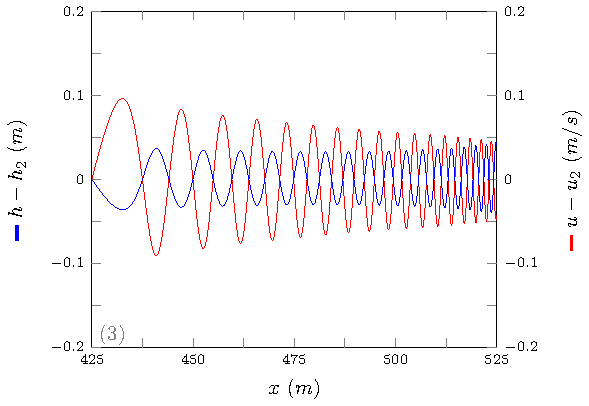
\includegraphics[width=0.5\textwidth]{pics/results/SDB/numsols/SWWCOMP/30s/1.pdf}
		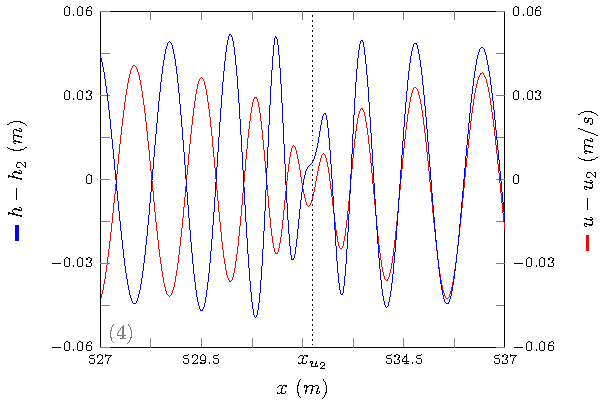
\includegraphics[width=0.5\textwidth]{pics/results/SDB/numsols/SWWCOMP/30s/3.pdf}
	\end{subfigure}
	\caption{$h - h_2$ ({\color{blue} \solidrule}) and $u - u_2$ ({\color{red} \solidrule}) for numerical solution of the smooth dam-break by $\mathcal{V}_3$ with $\alpha = 0.1m$ and $\Delta x = 10/2^{9}m$ at $t=30s$ as in Figure \ref{fig:o3a20dxlimcdexp}.}
	\label{fig:UHSWWcomp30sall}
\end{figure}

\begin{figure}
	\centering
\begin{subfigure}{\textwidth}
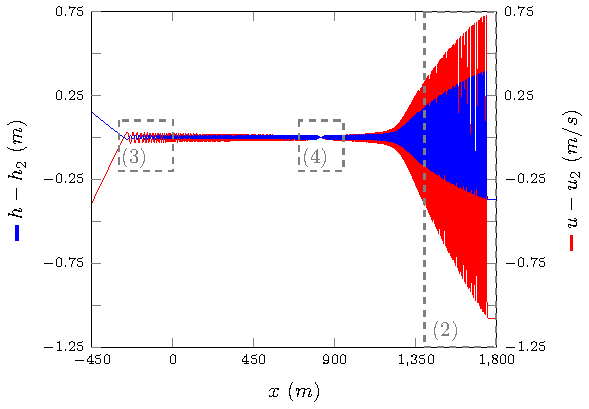
\includegraphics[width=0.5\textwidth]{pics/results/SDB/numsols/SWWCOMP/300s/0.pdf}
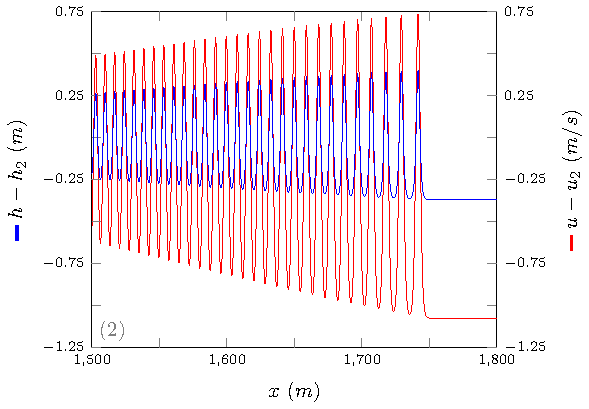
\includegraphics[width=0.5\textwidth]{pics/results/SDB/numsols/SWWCOMP/300s/2.pdf}
\end{subfigure}
\begin{subfigure}{\textwidth}
	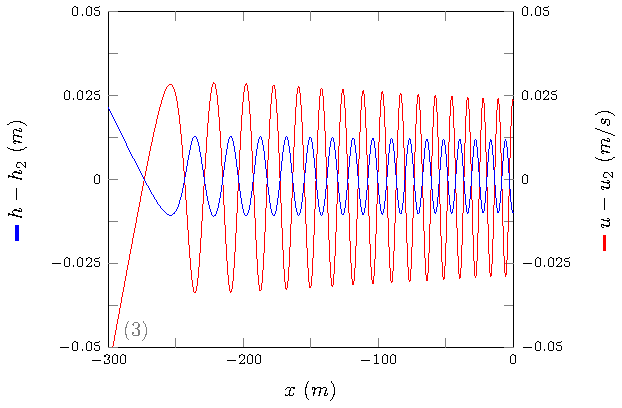
\includegraphics[width=0.5\textwidth]{pics/results/SDB/numsols/SWWCOMP/300s/1.pdf}
	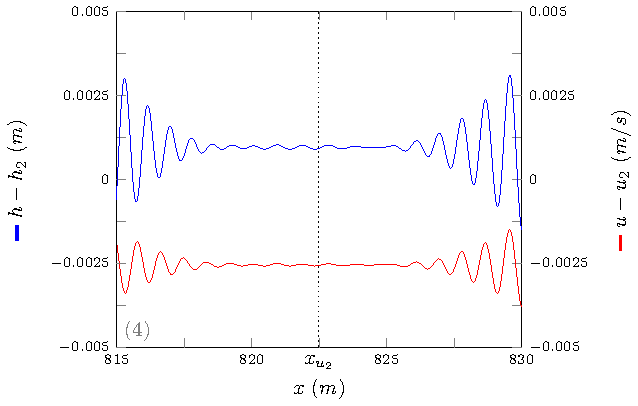
\includegraphics[width=0.5\textwidth]{pics/results/SDB/numsols/SWWCOMP/300s/3.pdf}
\end{subfigure}
	\caption{$h - h_2$ ({\color{blue} \solidrule}) and $u - u_2$ ({\color{red} \solidrule}) for numerical solution of the smooth dam-break by  $\mathcal{V}_3$ with $\alpha = 0.1m$ and $\Delta x = 10/2^{9}m$ at $t=300s$ as in Figure \ref{fig:FVcomplonga20}.}
	\label{fig:UHSWWcomp300sall}
\end{figure}

From Figure \ref{fig:UHSWWcomp30sall} and Figure \ref{fig:UHSWWcomp300sall} it can be seen that to the left of $x_{u_2}$ $u$ and $h$ are anti-phase while to the right of $x_{u_2}$ $u$ and $h$ are in-phase. The contact discontinuity \cite{El-etal-2006} marks the transition between these two states which is located at about $x_{u_2}$. Figure \ref{fig:UHSWWcomp300sall} demonstrates that at $x_{u_2}$, $h$ and $u$ are in-phase therefore the contact discontinuity is to the left of $x_{u_2}$, thus the speed of the contact discontinuity like the mean bore velocity is slightly overestimated by $u_2$. 

%%dispersion relation
Because $h$ and $u$ are anti-phase to the left of the contact discontinuity they appear to travel leftwards relative to it while those on the right are in-phase and therefore appear to travel rightwards relative to the contact discontinuity. Thus these oscillations appear to be forming at the contact discontinuity and then travelling away from it. The phase velocity of the linearised Serre equations is 
\[\upsilon_p = u \pm \sqrt{gh} \sqrt{\frac{3}{h^2 k^2 + 3}} \; \]
where $k$ is the wave number. The phase velocity has the following behaviour, as $k \rightarrow \infty$ then $\upsilon_p \rightarrow u$ and as $k \rightarrow 0$ then $\upsilon_p \rightarrow u \pm \sqrt{gh}$ . Since we observe $u$ and $h$ as being anti-phase to the left of the contact discontinuity this means we are in the negative branch of the phase velocity $u - \sqrt{gh} \sqrt{\frac{3}{h^2 k^2 + 3}}$ while the in-phase right side corresponds to the positive branch  $u + \sqrt{gh} \sqrt{\frac{3}{h^2 k^2 + 3}}$. Thus the contact discontinuity corresponds to oscillations with very high wave numbers, which are sensitive to both smoothing of the initial conditions and numerical diffusion.
%cd speed
By this phase velocity argument the contact discontinuity should travel at the mean bore velocity which is close to $u_2$ for a range of dam-break problems. To investigate this $h_0=1m$ was fixed and $h_1$ was varied to allow for different aspect ratios and thus different bore speeds. The results are plotted in Figure \ref{fig:CDspeed} from which it is quite clear that the contact discontinuity does in fact travel at close to $u_2$ for a range of aspect ratios. 
\begin{figure}
	\centering
	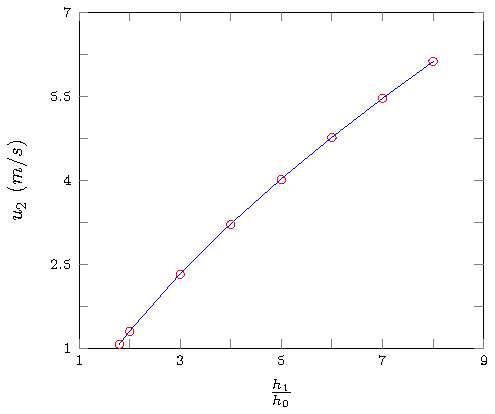
\includegraphics[width=0.5\textwidth]{pics/results/SDB/CDspeed/speed.pdf}
	\caption{$u_2$ ({\color{blue} \solidrule}) and speed of the contact discontinuity ({\color{red} $\circ$})  for numerical solutions of smoothed dam-break problems with different aspect ratios ($h_1 /h_0$) by $\mathcal{V}_3$ where $\alpha = 0.1m$ and $\Delta x = 10/2^{9}m$ at $t=100s$.}
	\label{fig:CDspeed}
\end{figure}


%%% a plus 
\subsubsection{Whitham modulation comparison}
The expressions for the leading wave amplitude $A^+$ and speed $S^+$ obtained by \citeN{El-etal-2006} are asymptotic results and so we are interested in how our numerical results behave over time. Thus for the dam-break problem in Figure \ref{fig:FVcomplonga20} the peak amplitude in region IV ($A$) was plotted over time in Figure \ref{fig:FVlonga20aplus}. From the figure it can see that $A$ approaches a value larger than $A^+$. We find that as $\alpha \rightarrow 0$ and $\Delta x \rightarrow 0$ our $A$ values converge away from $A^+$ not towards it in this time scale for this aspect ratio. Thus it appears that the true solution of the dam-break for the Serre equations has an amplitude in region IV slighlty above $A^+$. This is not inconsistent with the results of \cite{El-etal-2006} as their scale comparing $A^+$ to numerical solutions is too large to see such a small difference. From Figure \ref{fig:FVcomplonga20} it can be seen that while $S^+$ does not precisely predict the bore speed it is a better prediction than $S_2$.
\begin{figure}
	\centering
    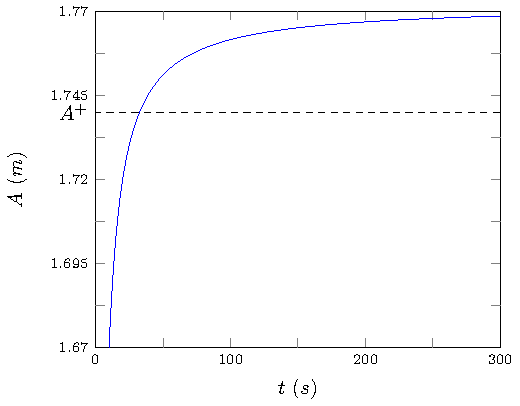
\includegraphics[width=0.5\textwidth]{pics/results/SDB/numsols/300s/a.pdf}
	\caption{Leading wave height plotted over time for the numerical solution of the smooth dam-break problem by $\mathcal{V}_3$ with $\alpha = 0.1m$ for $\Delta x = 10/2^{9}m$ ({\color{blue} \solidrule}) as in Figure \ref{fig:FVcomplonga20}.}
	\label{fig:FVlonga20aplus}
\end{figure}

%energy break down
\subsubsection{Energy Breakdown}
The Hamiltonian \eqref{eqn:Hamildef} has $3$ terms representing in order, horizontal kinetic energy $hu^2$, vertical kinetic energy $\frac{h^3}{3}\frac{\partial u}{\partial x}$ and gravitational potential energy $gh^2$. It might be expected that the oscillations of the undular bore such as in Figure \ref{fig:FVcomplonga20} would result in significant vertical energies. However, Figure \ref{fig:PHTa12all} demonstrates that this is not the case, as the total vertical kinetic energy in the system is insignificant relative to the other energies. This plot also demonstrates that even with dispersive terms and large oscillations the drivers of change in the dam-break problem are the transfer of gravitational potential energy into horizontal kinetic energy which occurs slowly.

\begin{figure}
	\centering
	\begin{subfigure}{\textwidth}
		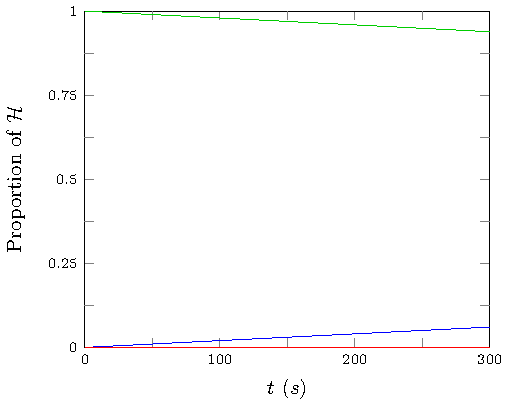
\includegraphics[width=0.5\textwidth]{pics/results/SDB/H/Time/HFT-figure0.pdf}
		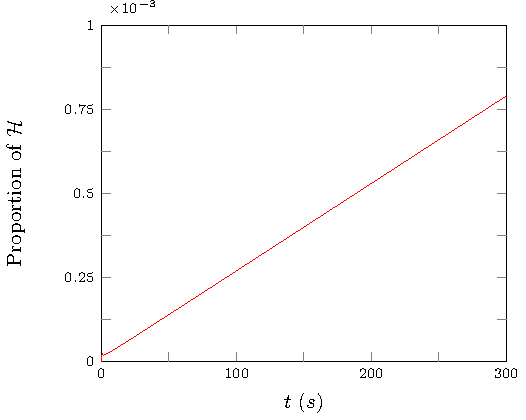
\includegraphics[width=0.5195\textwidth]{pics/results/SDB/H/Time/TT-figure0.pdf}
	\end{subfigure}
	\caption{Proportion of $\mathcal{H}$ made up by horizontal kinetic energy ({\color{blue} \solidrule}), vertical kinetic energy ({\color{red} \solidrule}) and gravitational potential energy ({\color{green!80!black} \solidrule}) for $\mathcal{V}_3$'s solution of the smooth dam-break problem with $\alpha = 0.1m$ and $\Delta x = 10/2^{9}m$ over time as in Figure \ref{fig:FVcomplonga20}.}
	\label{fig:PHTa12all}
\end{figure}
%--------------------------------------------------------------------------------
\section{Conclusions}
\label{section:Conclusions}
%--------------------------------------------------------------------------------
Utilising two finite difference methods of second-order and three finite difference-volume hybrid methods of various orders an investigation into the smoothed dam-break problem with varying steepness was performed. Four different behaviours were uncovered with the general trend being that an increase in steepness increases the size and number of oscillations in the solution. This study explains all current differences in the literature involving the solution of the Serre equations applied to the smoothed dam-break problem and also uncovers a new result. We find that while the analytic solution of the shallow water wave equations for the dam-break problem is a good guide to the mean behaviour of the Serre equations the speed and height of the bores do not match up precisely. While the Whitham modulation results for the Serre equations give better predictions than the shallow water wave equations analytic solution it was found that they also do not line up with our numerical results precisely. It was demonstrated that the contact discontinuity corresponds to high wave numbers and thus travels at the mean velocity inside the bore. It was also found that vertical kinetic energy is negligible for the dam-break problem. 

%more research

%--------------------------------------------------------------------------------
\bibliography{Serre_ASCE}
%--------------------------------------------------------------------------------

\end{document}
